\documentclass[a4paper]{article}

\usepackage{t1enc}
\usepackage[latin1]{inputenc}
\usepackage[english]{babel}
\usepackage{amsmath,amssymb,amsthm}
\usepackage{graphicx}
\usepackage{float}
\usepackage{url}

\usepackage[round]{natbib}
\bibliographystyle{plainnat}

\usepackage{hyperref}

\pagestyle{plain}
\setlength{\parindent}{0in}
\setlength{\parskip}{1.5ex plus 0.5ex minus 0.5ex}
\setlength{\oddsidemargin}{0in}
\setlength{\evensidemargin}{0in}
\setlength{\topmargin}{-0.5in}
\setlength{\textwidth}{6.3in}
\setlength{\textheight}{9.8in}

\numberwithin{equation}{section}
\newcommand\email{\begingroup \urlstyle{rm}\Url}

\theoremstyle{definition}
\newtheorem{defi}{Definition}[subsection]

\usepackage{/usr/lib/R/share/texmf/Sweave}
\begin{document}

%\VignetteIndexEntry{An R Package for Univariate and Bivariate Peaks  Over Threshold Analysis} 
%\VignetteDepens{POT}
%\VignetteKeyword{Extreme Value Theory, Multivariate Extremes} 
%\VignettePackage{POT}

\begin{center}
  \LARGE 
  A User's Guide to the POT Package (Version 1.1) \\
  \Large
  \vspace{0.2cm}
  Mathieu Ribatet \\
  \normalsize
  Copyright \copyright 2006 \\
  \vspace{0.2cm}
  Department of Hydrological Statistic, INRS,\\
  University of Qu\'ebec, 490 de la Couronne, G1K 9A9 Canada\\
  \vspace{0.2cm}
  Cemagref UR HH, 3bis quai Chauveau\\ 69336 Lyon Cedex
  09 France\\ 
  \vspace{0.2cm}
  E-mail: \email{ribatet@hotmail.com} \\
  17th October 2006
\end{center}

\section{Introduction}
\label{sec:intro}

\subsection{Why the POT package?}
\label{subsec:why}

The \textbf{POT} package is an add-on package for the R statistical
software~\citep{Rsoft}. The main goal of this package is to develop
tools to perform stastical analyses of Peaks Over a Threshold
(\textbf{POT}).

Most of functions are related to the Extreme Value Theory
(\textbf{EVT}). \citet{Coles2001} gives a comprehensive introduction
to the EVT, while~\citet{Kluppelberg1997} present advanced results.

\subsection{Obtaining the package/guide}

The package can be downloaded from CRAN (The Comprehensive R Archive
Network) at \url{http://cran.r-project.org/}.  This guide (in pdf)
will be in the directory \verb+POT/doc/+ underneath wherever the
package is installed.

\subsection{Contents}
\label{subsec:contents}

To help users to use properly the \textbf{POT} package, this guide
contains practical examples on the use of this
package. Section~\ref{sec:introEVT} introduce quickly the Extreme
Value Theory (\textbf{EVT}). Some basic examples are described in
section~\ref{sec:BasicUse}, while section~\ref{sec:concAn} gives a
concrete statistical analysis of extreme value for river Adie\'eres at
Beaujeu (FRANCE).

\subsection{Citing the package/guide}

To cite this guide or the package in publications please use the
following bibliographic database entry.
\begin{verbatim}
  title = {A User's Guide to the POT Package (Version 1.0)},
  author = {Ribatet, M. A.},
  year = {2006},
  month = {August},
  url = {http://cran.r-project.org/}
}
\end{verbatim}

\subsection{Caveat}

I have checked these functions as best I can but, as ever, they may
contain bugs.  If you find a bug or suspected bug in the code or the
documentation please report it to me at \verb+ribatet@hotmail.com+.
Please include an appropriate subject line.

\subsection{Legalese}

This program is free software; you can redistribute it and/or modify
it under the terms of the GNU General Public License as published by
the Free Software Foundation; either version 2 of the License, or (at
your option) any later version.

This program is distributed in the hope that it will be useful, but
without any warranty; without even the implied warranty of
merchantability or fitness for a particular purpose.  See the GNU
General Public License for more details.

The GNU General Public License can be obtained from
\url{http://www.gnu.org/copyleft/gpl.html}.  You can also obtain it by
writing to the Free Software Foundation, Inc., 59 Temple Place --
Suite 330, Boston, MA 02111-1307, USA.

\section{An Introduction the EVT}
\label{sec:introEVT}

\subsection{The univariate case}
\label{subsec:univ}

Even if this package is only related to peaks over a threshold, a
classical introduction to the EVT must deal with ``block maxima''. Let
$X_1,\ldots,X_n$ be a series of independent and identically distributed
random variables with commom distribution function $F$. Let $M_n =
\max(X_1,\ldots,X_n)$.

Suppose there exists normalizing constants $a_n>0$ and $b_n$ such
that:
\begin{equation}
  \label{eq:convMax}
  \Pr\left[\frac{M_n - b_n}{a_n} \leq y \right] = F^n(a_ny+b_n)
  \longrightarrow G(y), \qquad n \rightarrow +\infty
\end{equation}
for all $y \in \mathbb{R}$, where $G$ is a non-degenerate distribution
function. According to the Extremal Types Theorem~\citep{Fisher1928},
$G$ must be either Fr\'echet, Gumbel or negative
Weibull. \citet{Jenkinson1955} noted that these three distributions can
be merged into a single parametric family: the Generalized Extreme
Value (\textbf{GEV}) distribution. The GEV has a distribution function
defined by:
\begin{equation}
  \label{eq:GEV}
  G(y) = \exp\left[ -\left( 1 + \xi \frac{y-\mu}{\sigma}
    \right)_+^{-1/\xi} \right],
\end{equation}
where $(\mu,\sigma,\xi)$ are the location, scale and shape parameters
respectively, $\sigma>0$ and $z_+=\max(z,0)$.

The Fr\'echet case is obtained when $\xi>0$, the negative Weibull when
$\xi<0$ while the Gumbel case is defined by continuity when
$\xi\rightarrow0$.

From this result, \citet{Pickands1975} showed that the limiting
distribution of normalized excesses of a threshold $\mu$ as the
threshold approaches the endpoint $\mu_\mathrm{end}$ of the variable
of interest is the Generalized Pareto Distribution
(\textbf{GPD}). That is, if $X$ is a random variable which
holds~\eqref{eq:convMax}, then:
\begin{equation}
  \label{eq:convExcess}
  \Pr\left[X \leq y | X > \mu \right] \longrightarrow H(y), \qquad \mu
    \rightarrow \mu_\mathrm{end}
\end{equation}
with
\begin{equation}
  \label{eq:GPD}
  H(y) = 1 - \left(1 + \xi\frac{y-\mu}{\sigma}\right)_+^{-1/\xi},
\end{equation}
where $(\mu,\sigma,\xi)$ are the location, scale and shape parameters
respectively, $\sigma>0$ and $z_+=\max(z,0)$. Note that the
Exponential distribution is obtained by continuity as $\xi \rightarrow
0$.

In practice, these two asymptotical results motivated modelling block
maxima with a GEV, while peaks over threshold with a GPD.

\subsection{The multivariate case}
\label{subsec:multiv}

When dealing with multivariate extremes, it is usual to transform data
to a particular distribution. For example, \citet{Falk2005} used the
inverted standard exponential distribution -- $\Pr[Z \leq z ] =
\exp(z)$, $z \leq 0$, \citet{Coles1999} use the uniform distribution
on $[0,1]$. However, the most common distribution seems to be the
standard Fr\'echet one -- $\Pr[Z \leq z] = \exp(-1/z)$
\citep{Smith1994,Smith1997,Bortot2000}. Thus, in the following, we
will only consider this case. For this purpose, margins are
transformed according to:
\begin{displaymath}
  Z_j = - \frac{1}{\log F_j \left( Y_j \right)}
\end{displaymath}
where $F_j$ is the distribution of the $j$-th margin.

Obviously, in practice, the margins $F_j$ are unknown. When dealing
with extremes, the univariate EVT tells us what to do. Thus, if block
maxima or peaks over a threshold are of interest, we must replace
$F_j$ with GEV or GPD respectively.

\begin{defi}
  A multivariate extreme value distribution in dimension $d$ has
  representation:
  \begin{equation}
    \label{eq:expMesRep}
    G\left(y_1, \ldots, y_d \right) = \exp\left[-V\left(z_1, \ldots,
        z_d \right) \right]
  \end{equation}
  with
  \begin{displaymath}
    V(z_1, \ldots, z_d) = \int_{T_p} \max_{j=1,\ldots,d}
    \left(\frac{q_j}{z_j} \right) \mbox{dH}\left(q_1,
      \ldots,q_d\right) 
  \end{displaymath}
  where $H$ is a measure with mass 2 called \emph{spectral density}
  defined on the set
  \begin{displaymath}
    T_p = \left\{ \left(q_1, \ldots, q_d \right) : q_j \geq 0,
    \sum_{j=1}^d q_j^2 = 1 \right\}
  \end{displaymath}
  with the constraint
  \begin{displaymath}
    \int_{T_p} q_jdH(q_j) = 1, \qquad \forall j \in \left\{1, \ldots,
      d\right\}
  \end{displaymath}
\end{defi}

The $V$ function is often called \emph{exponential
  measure}~\citep{Kluppelberg2006} and is an homogeneous function of
order -1.

Contrary to the univariate case, there is an infinity of functions $V$
for $d>1$. Thus, it is usual to used specific parametric families for
$V$. Several examples for these families are given in
Annexe~\ref{sec:copula}.

Another representation for a multivariate extreme value distribution
is the Pickands' representation~\citep{Pickands1981}. We give here
only the bivariate case.

\begin{defi}
  A bivariate extreme value distribution has the Pickands' representation:
  \begin{equation}
    \label{eq:pickDepRep}
    G\left(y_1, y_2 \right) = \exp\left[- \left(\frac{1}{z_1} +
        \frac{1}{z_2} \right) A\left( \frac{z_2}{z_1+z_2} \right)
    \right]
  \end{equation}
  with
  \begin{eqnarray*}
    A : \left[0, 1 \right] &\longrightarrow& \left[0, 1 \right]\\
    w &\longmapsto& A(w) = \int_0^1 \max\left\{w\left(1-q\right),
      \left(1-w \right)q \right\} dH(q)
  \end{eqnarray*}
\end{defi}

In particular, the functions $V$ and $A$ are linked by the relation:
\begin{displaymath}
  A(w) = \frac{V\left(z_1,z_2\right)}{z_1^{-1} + z_2^{-1}},
  \qquad w = \frac{z_2}{z_1 + z_2}
\end{displaymath}

The dependence function $A$ holds:
\begin{enumerate}
\item $A(0) = A(1) = 1$;
\item $\max(w, 1 -w) \leq A(w) \leq 1$, $\forall w$;
\item $A$ is convex;
\item Two random variables (with unit Fr\'echet margins) are
  independent if $A(w)=1$, $\forall w$; 
\item Two random variables (with unit Fr\'echet margins) are
  perfectly dependent if $A(w)=\max(w,1-w)$, $\forall w$. 
\end{enumerate}

We define the multivariate extreme value distributions which are
identical to the block maxima approach in higher dimensions. We now
establish the multivariate theory for peaks over threshold.

According to~\citet[Prop. 5.15]{Resnick1987}, multivariate peaks over
thresholds $u_j$ has the same representation than for block
maxima. Only the margins $F_j$ must be replaced by GPD instead of
GEV\@. Thus,
\begin{equation}
  \label{eq:multExcess}
  F\left(y_1, \ldots, y_d \right) = \exp\left[-V\left( - \frac{1}{\log
      F_1\left(y_1 \right)}, \ldots, - \frac{1}{\log F_d\left(y_d
      \right)} \right) \right], \qquad y_j > u_j
\end{equation}

 
\section{Basic Use}
\label{sec:BasicUse}

\subsection{Random Numbers and Distribution Functions}
\label{subsec:randDist}

First of all, lets start with basic stuffs. The \textbf{POT} package
uses the R convention for random numbers generation and distribution
function features. 

\begin{Schunk}
\begin{Sinput}
> library(POT)
> rgpd(5, loc = 1, scale = 2, shape = -0.2)
\end{Sinput}
\begin{Soutput}
[1] 1.665971 3.760271 1.379118 1.350935 2.809759
\end{Soutput}
\begin{Sinput}
> rgpd(6, c(1, -5), 2, -0.2)
\end{Sinput}
\begin{Soutput}
[1]  1.584634 -3.317012  1.467413 -3.970143  1.614645 -2.568265
\end{Soutput}
\begin{Sinput}
> rgpd(6, 0, c(2, 3), 0)
\end{Sinput}
\begin{Soutput}
[1] 2.259214 1.396235 1.153899 1.195256 1.754853 1.753172
\end{Soutput}
\begin{Sinput}
> pgpd(c(9, 15, 20), 1, 2, 0.25)
\end{Sinput}
\begin{Soutput}
[1] 0.9375000 0.9825149 0.9922927
\end{Soutput}
\begin{Sinput}
> qgpd(c(0.25, 0.5, 0.75), 1, 2, 0)
\end{Sinput}
\begin{Soutput}
[1] 1.575364 2.386294 3.772589
\end{Soutput}
\begin{Sinput}
> dgpd(c(9, 15, 20), 1, 2, 0.25)
\end{Sinput}
\begin{Soutput}
[1] 0.015625000 0.003179117 0.001141829
\end{Soutput}
\end{Schunk}

Several options can be passed to three of these four functions. In
particular:
\begin{itemize}
\item for ``pgpd'', user can specify if non exceedence or exceedence
  probability should be computed with option \verb+lower.tail = TRUE+
  or  \verb+lower.tail = FALSE+ respectively;
\item for ``qgpd'', user can specify if quantile is related to non
  exceedence or exceedence probability with option
  \verb+lower.tail = TRUE+ or \verb+lower.tail = FALSE+ respectively;
\item for ``dgpd'', user can specify if the density or the log-density
  should be computed with option \verb+log = FALSE+ or
  \verb+log = TRUE+ respectively.
\end{itemize}

\subsection{Threshold Selection}
\label{subsec:threshSelect}

The location for the GPD or equivalently the threshold is a particular
parameter as must often it is not estimated as the other ones. All
methods to define a suitable threshold use the asymptotic
approximation defined by equation~\eqref{eq:convExcess}. In other
words, we select a threshold for which the asymptotic distribution $H$
in equation~\eqref{eq:GPD} is a good approximation.

The \textbf{POT} package has several tools to define a reasonable
threshold. For this purpose, the user must use
\verb+tcplot, mrlplot, lmomplot, exiplot+ and \verb+diplot+ functions.

The main goal of threshold selection is to selects enough events to
reduce the variance; but not too much as we could select events coming
from the central part of the distribution\footnote{i.e.\ not extreme
  events.} and induce bias.

\subsubsection{Threshold Choice plot:  \emph{tcplot}}
\label{subsubsection:tcplot}

Let $X \sim GP(\mu_0, \sigma_0, \xi_0)$. Let $\mu_1$ be a another
threshold as $\mu_1 > \mu_0$. The random variable $X | X > \mu_1$ is
also GPD with updated parameters $\sigma_1 = \sigma_0 + \xi_0 ( \mu_1
- \mu_0)$ and $\xi_1 = \xi_0$.
Let
\begin{equation}
  \label{eq:reparamScale}
  \sigma_* = \sigma_1 - \xi_1 \mu_1
\end{equation}
With this new parametrization, $\sigma_*$ is independent of
$\mu_1$. Thus, estimates of $\sigma_*$ and $\xi_1$ are constant for
all $\mu_1 > \mu_0$ if $\mu_0$ is a suitable threshold for the
asymptotic approximation.

Threshold choice plots represent the points defined by:
\begin{equation}
  \label{eq:tcplot}
  \left\{\left(\mu_1, \sigma_*\right) : \mu_1 \leq x_\mathrm{max}
  \right\} \quad \text{and} \quad \left\{\left(\mu_1, \xi_1\right) :
    \mu_1 \leq x_\mathrm{max} \right\}
\end{equation}
where $x_\mathrm{max}$ is the maximum of the observations
$\mathbf{x}$.

Moreover, confidence intervals can be computed using Fisher
information. 

Here is an application.
\begin{Schunk}
\begin{Sinput}
> x <- runif(10000)
\end{Sinput}
\end{Schunk}

\begin{Schunk}
\begin{Sinput}
> par(mfrow = c(1, 2))
> tcplot(x, u.range = c(0.9, 0.995))
\end{Sinput}
\end{Schunk}

\begin{figure}
\begin{center}
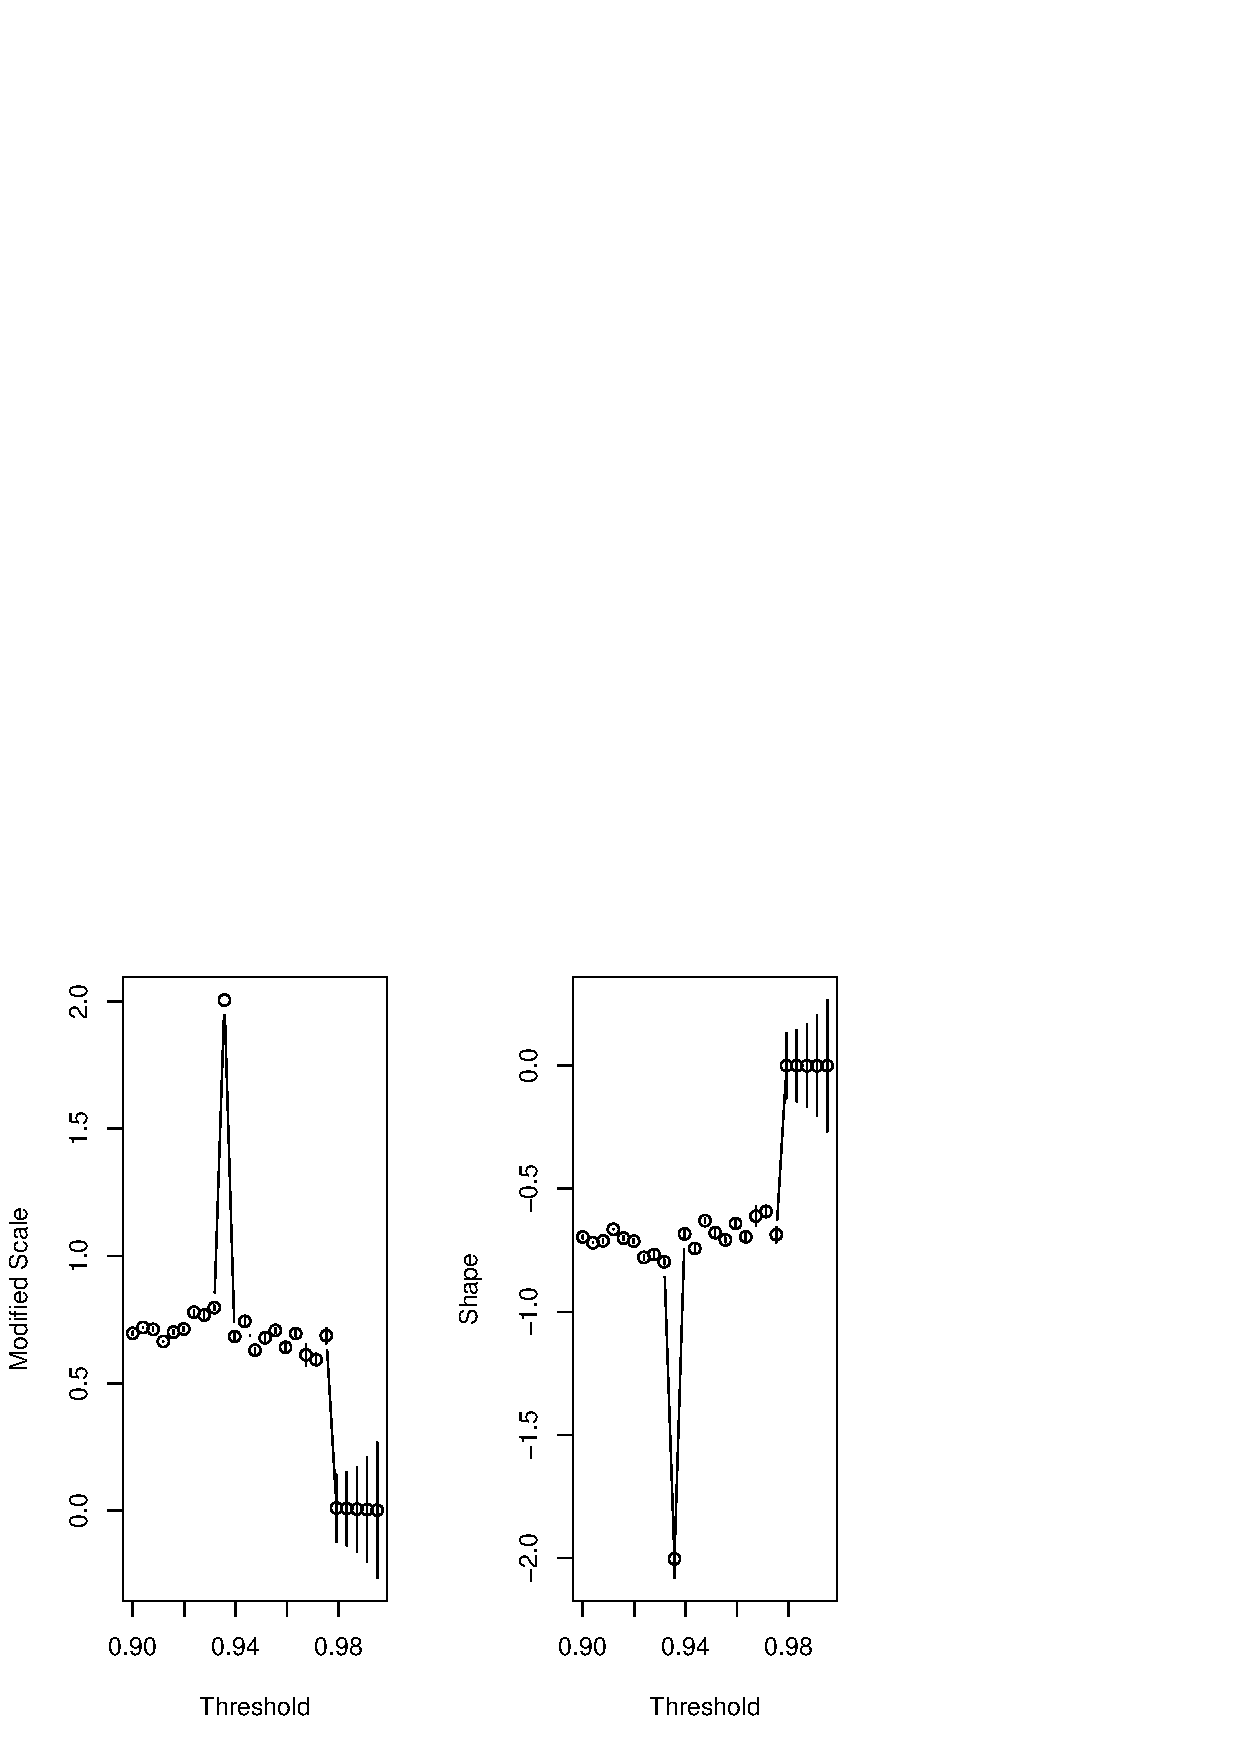
\includegraphics{guide-004}
\end{center}
\caption{The threshold selection using the tcplot function}
\label{fig:tcplot}
\end{figure}

Results of the \verb+tcplot+ function is displayed in
Figure~\ref{fig:tcplot}. We can see clearly that a threshold around
0.98 is a reasonable choice. However, in practice decision are not so
clear-cut as for this synthetic example.


\subsubsection{Mean Residual Life Plot: \emph{mrlplot}}

The \textbf{mean residual life plot} is based on the theoretical mean
of the GPD\@. Let $X$ be a \textit{r.v.} distributed as $GPD(\mu,
\sigma, \xi)$. Then, theoretically we have:
\begin{equation}
  \label{eq:meanGPD}
  \mathbb{E}\left[X \right] = \mu + \frac{\sigma}{1-\xi}, \qquad
  \text{for } \xi < 1
\end{equation}
When $\xi\geq1$, the theoretical mean is infinite.

In practice, if $X$ represents excess over a threshold $\mu_0$, and if
the approximation by a GPD is good enough, we have:
\begin{equation}
  \label{eq:meanExcess}
  \mathbb{E}\left[X - \mu_0 | X > \mu_0 \right] =
  \frac{\sigma_{\mu_0}}{1 - \xi}
\end{equation}
For all new threshold $\mu_1$ such as $\mu_1 > \mu_0$, excesses above
the new threshold are also approximate by a GPD with updated
parameters - see section~\ref{subsubsection:tcplot}. Thus,
\begin{equation}
  \label{eq:meanExcess2}
  \mathbb{E}\left[X - \mu_1 | X > \mu_1 \right] =
  \frac{\sigma_{\mu_1}}{1 - \xi} = \frac{\sigma_{\mu_0} +
    \xi \mu_1}{1 - \xi}
\end{equation}
The quantity $\mathbb{E}\left[X - \mu_1 | X > \mu_1 \right]$ is linear
in $\mu_1$. Or, $\mathbb{E}\left[X - \mu_1 | X > \mu_1 \right]$ is
simply the mean of excesses above the threshold $\mu_1$ which can
easily be estimated using the empirical mean.

A mean residual life plot consists in representing points:
\begin{equation}
  \label{eq:mrlplot}
  \left\{\left(\mu, \frac{1}{n_\mu} \sum_{i=1}^{n_\mu} x_{i, n_\mu} -
      \mu \right) : \mu \leq x_\mathrm{max} \right\}
\end{equation}
where $n_\mu$ is the number of observations $\mathbf{x}$ above the
threshold $\mu$, $x_{i, n_\mu}$ is the $i$-th observation above the
threshold $\mu$ and $x_\mathrm{max}$ is the maximum of the
observations $\mathbf{x}$.

Confidence intervals can be added to this plot as the empirical mean
can be supposed to be normally distributed (Central Limit
Theorem). However, normality doesn't hold anymore for high threshold
as there are less and less excesses. Moreover, by construction, this
plot always converge to the point $(x_\mathrm{max}, 0)$.

Here is another synthetic example.
\begin{Schunk}
\begin{Sinput}
> x <- rnorm(10000)
\end{Sinput}
\end{Schunk}

\begin{Schunk}
\begin{Sinput}
> mrlplot(x, u.range = c(1, quantile(x, probs = 0.995)), col = c("green", 
+     "black", "green"), nt = 200)
\end{Sinput}
\end{Schunk}

\begin{figure}
\begin{center}
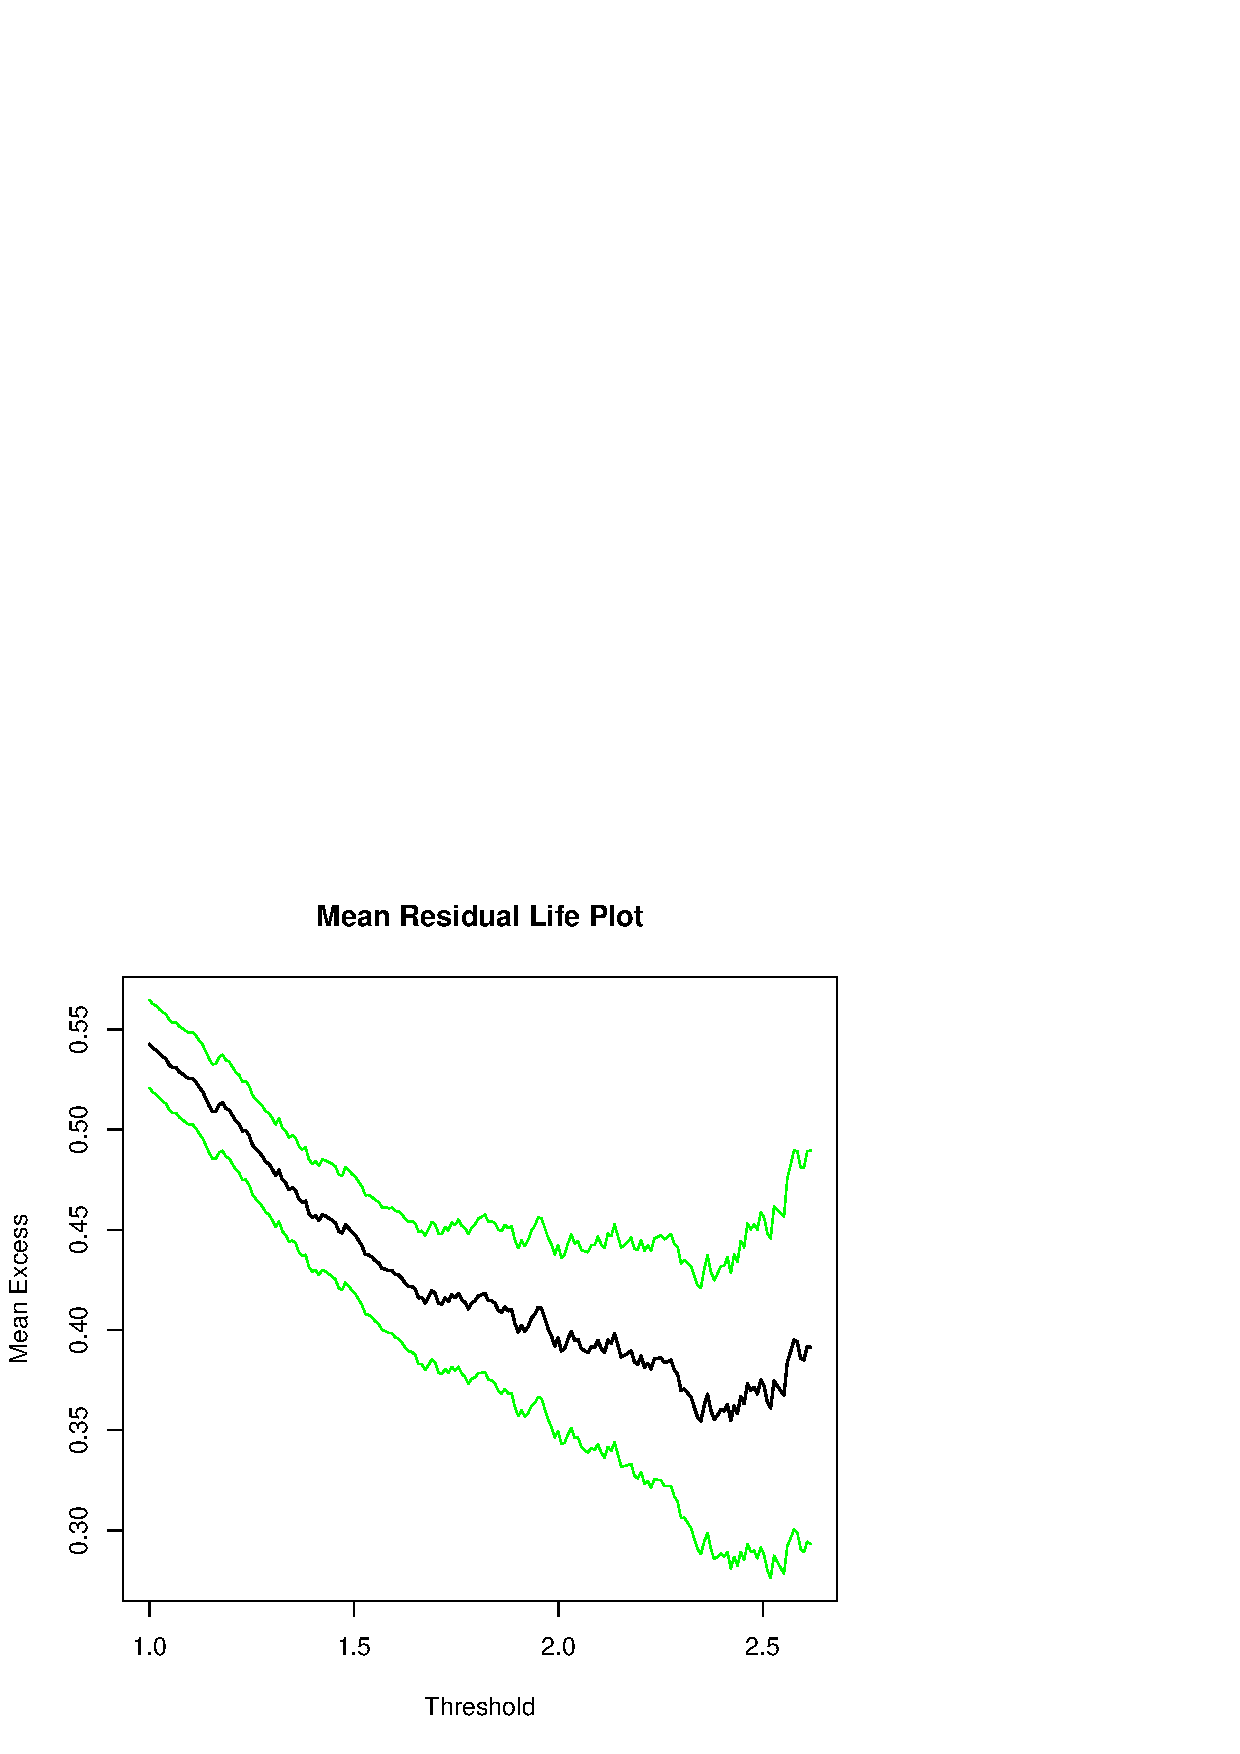
\includegraphics{guide-007}
\end{center}
\caption{The threshold selection using the mrlplot function}
\label{fig:mrlplot}
\end{figure}
 

Figure~\ref{fig:mrlplot} displays the mean residual life plot. A
threshold around 2.5 should be reasonable.


\subsubsection{L-Moments plot: \emph{lmomplot}}

L-moments are summary statistics for probability distributions and
data samples. They are analogous to ordinary moments -- they provide
measures of location, dispersion, skewness, kurtosis, and other
aspects of the shape of probability distributions or data samples --
but are computed from linear combinations of the ordered data values
(hence the prefix L).

For the GPD, the following relation holds:
\begin{equation}
  \label{eq:lomRel}
  \tau_4 = \tau_3 \frac{1 + 5 \tau_3}{5 + \tau_3}
\end{equation}
where $\tau_4$ is the \textbf{L-Kurtosis} and $\tau_3$ is the
\textbf{L-Skewness}.

The \textbf{L-Moment} plot represents points defined by:
\begin{equation}
  \label{eq:lmomplot}
  \left\{\left(\hat{\tau}_{3,u}, \hat{\tau}_{4,u}\right) : u \leq
    x_\mathrm{max} \right\}  
\end{equation}
where $\hat{\tau}_{3,u}$ and $\hat{\tau}_{4,u}$ are estimations of the
L-Kurtosis and L-Skewness based on excesses over threshold $u$ and
$x_\mathrm{max}$ is the maximum of the observations $\mathbf{x}$. The
theoretical curve defined by equation~\eqref{eq:lomRel} is traced as a
guideline.

Here is a trivial example.
\begin{Schunk}
\begin{Sinput}
> x <- c(1 - abs(rnorm(200, 0, 0.2)), rgpd(100, 1, 2, 0.25))
\end{Sinput}
\end{Schunk}
\begin{Schunk}
\begin{Sinput}
> lmomplot(x, u.range = c(0.9, quantile(x, probs = 0.9)), identify = FALSE)
\end{Sinput}
\end{Schunk}

\begin{figure}
\begin{center}
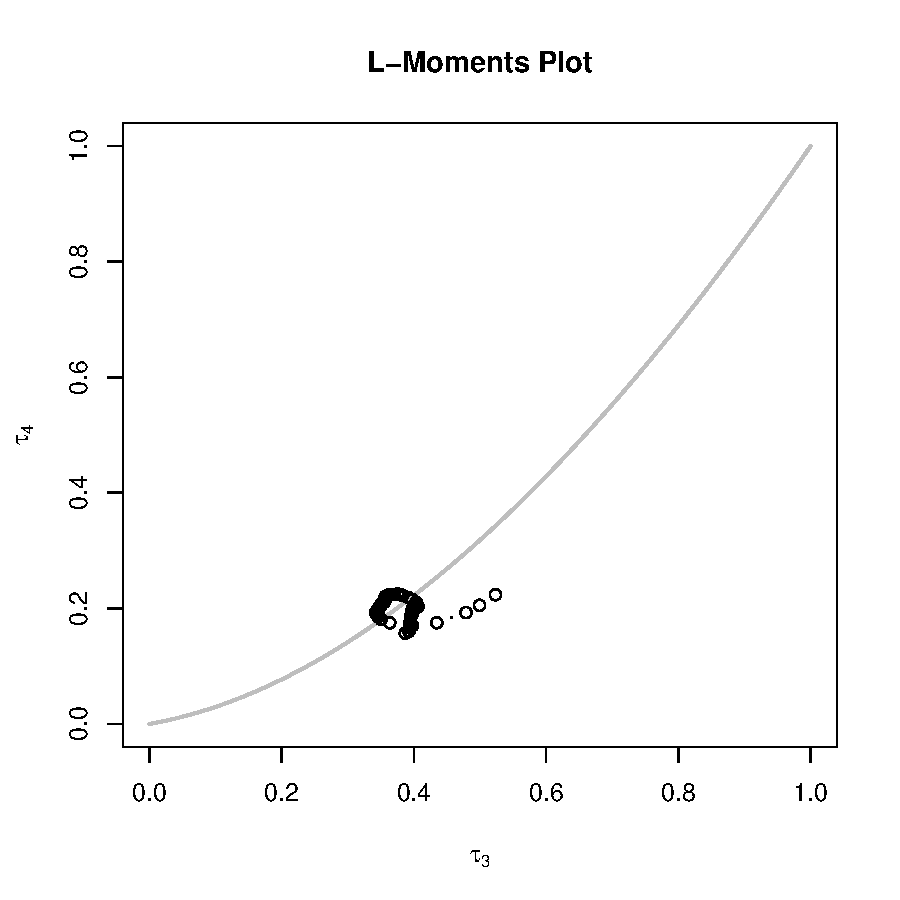
\includegraphics{guide-010}
\end{center}
\label{fig:lmomplot}
\caption{fig: The threshold selection using the lmomplot function}
\end{figure}

Figure~\ref{fig:lmomplot} displays the L-Moment plot. By passing
option \verb+identiy = TRUE+ user can click on the graphic to identify
the threshold related to the point selected.

We found that this graphic has often poor performance on real data.

\subsubsection{Dispersion Index Plot: \emph{diplot}}

The \textbf{Dispersion Index plot} is particularly useful when dealing
with time series. The EVT states that excesses over a threshold can be
approximated by a GPD\@. However, the EVT also states that the
occurrences of these excesses must be represented by a Poisson
process.

Let $X$ be a \textit{r.v.} distributed as a Poisson distribution with
parameter $\lambda$. That is:
\begin{equation}
  \label{eq:poissLaw}
  \Pr\left[X = k\right] = e^{-\lambda} \frac{\lambda^k}{k!}, \quad k
  \in \mathbb{N}.
\end{equation}
Thus, we have $\mathbb{E}\left[X\right] =
Var\left[X\right]$. \citet{Cunnane1979} introduced a
\textbf{Dispersion Index} statistic defined by:
\begin{equation}
  \label{eq:DI}
  DI = \frac{s^2}{\lambda}
\end{equation}
where $s^2$ is the intensity of the Poisson process and $\lambda$ the
mean number of events in a block - most often this is a
year. Moreover, a confidence interval can be computed by using a
$\chi^2$ test:
\begin{equation}
  \label{eq:confDI}
   I_{\alpha} = \left[ \frac{\chi^2_{\left(1 - \alpha\right) / 2,
        M-1}}{M-1}, \frac{\chi^2_{1 - \left( 1 -\alpha\right) / 2,
        M-1}}{M-1} \right]
\end{equation}
where $\Pr\left[ DI \in I_{\alpha} \right] = \alpha$.

For the next example, we use the data set \emph{ardieres} included in
the \textbf{POT} package. Moreover, as \emph{ardieres} is a time
series, and thus strongly auto-correlated, we must ``extract'' extreme
events while preserving independence between events. This is achieved
using function \textbf{clust}\footnote{The clust function will be
  presented later in section~\ref{subsec:declust}.}.

\begin{Schunk}
\begin{Sinput}
> data(ardieres)
> events <- clust(ardieres, u = 2, tim.cond = 8/365, clust.max = TRUE)
> diplot(events, u.range = c(2, 20))
\end{Sinput}
\end{Schunk}

\begin{figure}
\centering
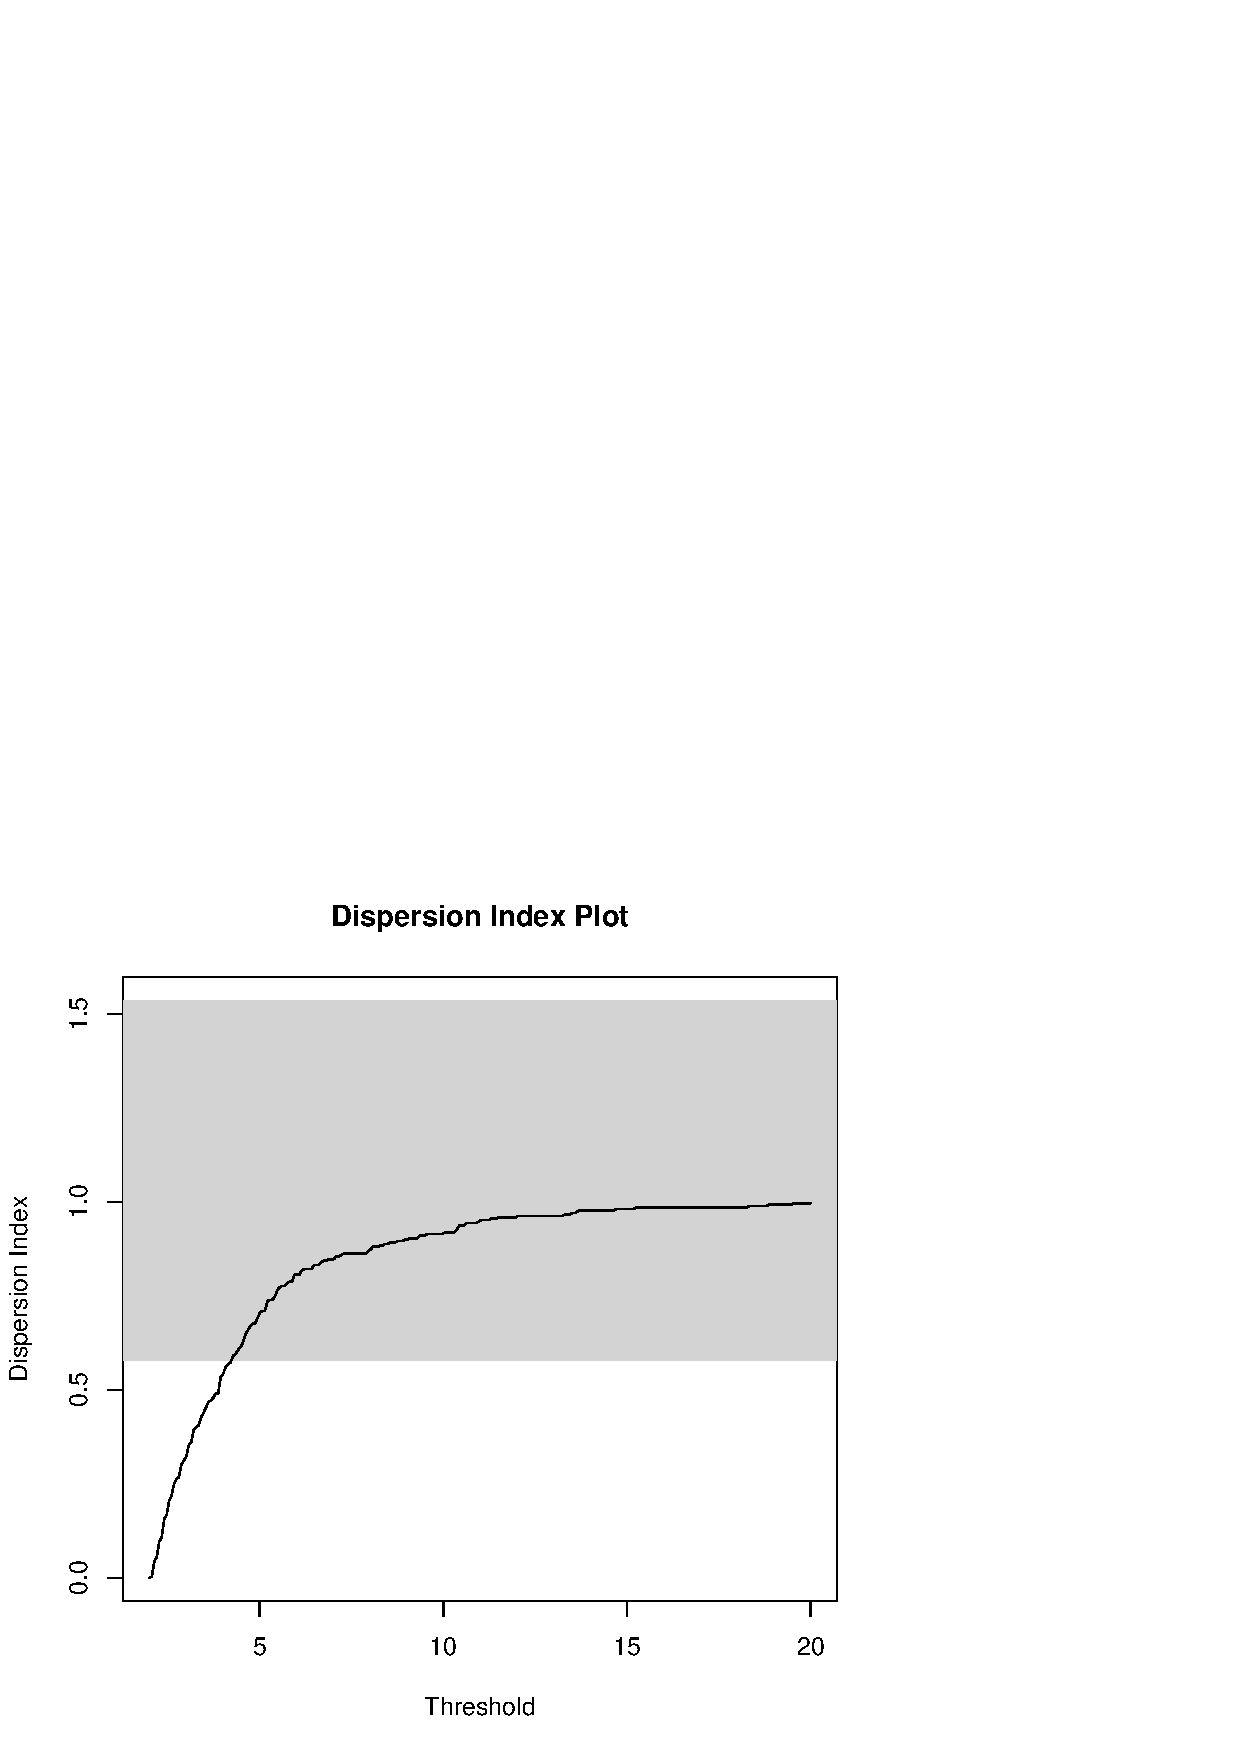
\includegraphics{guide-012}
\caption{The threshold selection using the diplot function}
\label{fig:diplot}
\end{figure}

The Dispersion Index plot is presented in
Figure~\ref{fig:diplot}. From this figure, a threshold around 5 should
be reasonable.

\subsection{Fitting the GPD}
\label{subsec:fitGPD}

\subsubsection{The univariate case}

The main function to fit the GPD is called \textbf{fitgpd}. This is a
generic function which can fit the GPD according several
estimators. There are currently 7 estimators available: method of
moments \verb|moments|, maximum likelihood \verb|mle|, biased and
unbiased probability weighted moments \verb|pwmb, pwmu|, mean power
density divergence \verb|mdpd|, median \verb|med| and pickands'
\verb|pickands| estimators. Details for these estimators can be found
in~\citep{Coles2001}, \citep{Hosking1987}, \citep{Juarez2004},
\citep{Peng2001} and \citep{Pickands1975}.

The MLE is a particular case as it is the only one which allows
varying threshold. Moreover, two types of standard errors are
available: ``expected'' or ``observed'' information of Fisher. The
option \verb|obs.fish| specifies if we want observed
(\verb|obs.fish = TRUE|) or expected (\verb|obs.fish = FALSE|).

As Pickands' estimator is not always feasible, user must check the
message of feasibility return by function \verb+fitgpd+.

We give here several didactic examples.
\begin{Schunk}
\begin{Sinput}
> x <- rgpd(200, 1, 2, 0.25)
> mom <- fitgpd(x, 1, "moments")$param
> mle <- fitgpd(x, 1, "mle")$param
> pwmu <- fitgpd(x, 1, "pwmu")$param
> pwmb <- fitgpd(x, 1, "pwmb")$param
> pickands <- fitgpd(x, 1, "pickands")$param
> med <- fitgpd(x, 1, "med", start = mle)$param
> mdpd <- fitgpd(x, 1, "mdpd")$param
> print(rbind(mom, mle, pwmu, pwmb, pickands, med, mdpd))
\end{Sinput}
\begin{Soutput}
            scale      shape
mom      2.392837 0.14165891
mle      2.253140 0.19668574
pwmu     2.215372 0.20531766
pwmb     2.226946 0.20116599
pickands 2.104060 0.23094281
med      2.262220 0.09430197
mdpd     2.219928 0.21650447
\end{Soutput}
\end{Schunk}

The MLE method allows to fix either the scale or the shape
parameter. For example, if we want to fit a Exponential distribution,
just do (with eventually a fixed scale parameter):

\begin{Schunk}
\begin{Sinput}
> x <- rgpd(100, 1, 2, 0)
> fitgpd(x, thresh = 1, shape = 0, method = "mle")
\end{Sinput}
\begin{Soutput}
Estimator: MLE 
Deviance: 340.4654 
     AIC: 342.4654 

Varying Threshold: FALSE 

Threshold Call: 1 
Number Above: 100 
Proportion Above: 1 

Estimates
scale  
2.018  

Standard Error Type: observed 

Standard Errors
 scale  
0.2018  

Asymptotic Variance Covariance
       scale  
scale  0.04074

Optimization Information
  Convergence: successful 
  Function Evaluations: 7 
  Gradient Evaluations: 1 
\end{Soutput}
\begin{Sinput}
> fitgpd(x, thresh = 1, scale = 2, method = "mle")
\end{Sinput}
\begin{Soutput}
Estimator: MLE 
Deviance: 338.8422 
     AIC: 340.8422 

Varying Threshold: FALSE 

Threshold Call: 1 
Number Above: 100 
Proportion Above: 1 

Estimates
  shape  
-0.0876  

Standard Error Type: observed 

Standard Errors
  shape  
0.05646  

Asymptotic Variance Covariance
       shape   
shape  0.003188

Optimization Information
  Convergence: successful 
  Function Evaluations: 19 
  Gradient Evaluations: 7 
\end{Soutput}
\end{Schunk}

If now, we want to fit a GPD with a varying threshold, just do:

\begin{Schunk}
\begin{Sinput}
> x <- rgpd(500, 1:2, 0.3, 0.01)
> fitgpd(x, 1:2, method = "mle")
\end{Sinput}
\begin{Soutput}
Estimator: MLE 
Deviance: -230.8703 
     AIC: -226.8703 

Varying Threshold: TRUE 

Threshold Call: c(1, 2) 
Number Above: 500 
Proportion Above: 1 

Estimates
   scale     shape  
 0.32118  -0.09512  

Standard Error Type: observed 

Standard Errors
  scale    shape  
0.02124  0.04892  

Asymptotic Variance Covariance
       scale       shape     
scale   0.0004513  -0.0008238
shape  -0.0008238   0.0023928

Optimization Information
  Convergence: successful 
  Function Evaluations: 75 
  Gradient Evaluations: 15 
\end{Soutput}
\end{Schunk}

Note that the varying threshold is repeated cyclically until it
matches the length of object \verb|x|.

\subsubsection{The bivariate case}

The generic function to fit bivariate POTs is \textbf{fitbvgpd}. There
is currently 6 models for the bivariate GPD -- see
Annexe~\ref{sec:copula}. All of these models are fitted using maximum
likelihood estimator. Moreover, the approach uses \emph{censored}
likelihood -- see \citep{Smith1997}.

\begin{Schunk}
\begin{Sinput}
> x <- rgpd(500, 0, 1, 0.25)
> y <- rgpd(500, 2, 0.5, -0.25)
> Mlog <- fitbvgpd(cbind(x, y), c(0, 2), model = "log")
> Mlog
\end{Sinput}
\begin{Soutput}
Call: fitbvgpd(data = cbind(x, y), threshold = c(0, 2), model = "log") 
Estimator: MLE 
Dependence Model and Strenght:
	Model : Logistic 
	lim_u Pr[ X_1 > u | X_2 > u] = 0.001 
Deviance: 1252.647 
     AIC: 1262.647 

Marginal Threshold: 0 2 
Marginal Number Above: 500 500 
Marginal Proportion Above: 1 1 
Joint Number Above: 500 
Joint Proportion Above: 1 
Number of events such as {Y1 > u1} U {Y2 > u2}: 500 

Estimates
 scale1   shape1   scale2   shape2    alpha  
 0.9739   0.2205   0.4887  -0.2343   0.9993  

Standard Errors
   scale1     shape1     scale2     shape2      alpha  
6.710e-02  5.250e-02  2.849e-02  3.877e-02  2.001e-06  

Asymptotic Variance Covariance
        scale1      shape1      scale2      shape2      alpha     
scale1   4.502e-03  -2.223e-03   1.544e-06  -1.146e-06   3.361e-12
shape1  -2.223e-03   2.757e-03  -5.312e-08   1.848e-07  -2.060e-11
scale2   1.544e-06  -5.312e-08   8.115e-04  -9.112e-04   3.879e-13
shape2  -1.146e-06   1.848e-07  -9.112e-04   1.503e-03  -1.392e-12
alpha    3.361e-12  -2.060e-11   3.879e-13  -1.392e-12   4.003e-12

Optimization Information
	Convergence: successful 
	Function Evaluations: 120 
	Gradient Evaluations: 14 
\end{Soutput}
\end{Schunk}

In the summary, we can see \verb+lim_u Pr[ X_1 > u | X_2 > u] = 0.02+
. This is the $\chi$ statistics of \citet{Coles1999}. For the
parametric model, we have:
\begin{displaymath}
  \chi = 2 - V(1,1) = 2 \left(1 - A(0.5) \right)
\end{displaymath}

For independent variables, $\chi = 0$ while for perfect dependence,
$\chi = 1$. In our application, the value 0.02 indicates that the
variables are independent -- which is obvious. In this perspective, it
is possible to fixed some parameters. For our purpose of independence,
we can run -which is equivalent to fit x and y separately of course:
\begin{Schunk}
\begin{Sinput}
> fitbvgpd(cbind(x, y), c(0, 2), model = "log", alpha = 1)
\end{Sinput}
\begin{Soutput}
Call: fitbvgpd(data = cbind(x, y), threshold = c(0, 2), model = "log",      alpha = 1) 
Estimator: MLE 
Dependence Model and Strenght:
	Model : Logistic 
	lim_u Pr[ X_1 > u | X_2 > u] = 0 
Deviance: 1252.572 
     AIC: 1260.572 

Marginal Threshold: 0 2 
Marginal Number Above: 500 500 
Marginal Proportion Above: 1 1 
Joint Number Above: 500 
Joint Proportion Above: 1 
Number of events such as {Y1 > u1} U {Y2 > u2}: 500 

Estimates
 scale1   shape1   scale2   shape2  
 0.9722   0.2308   0.4886  -0.2338  

Standard Errors
 scale1   shape1   scale2   shape2  
0.06773  0.05441  0.02851  0.03892  

Asymptotic Variance Covariance
        scale1      shape1      scale2      shape2    
scale1   4.588e-03  -2.325e-03  -6.048e-14   1.001e-13
shape1  -2.325e-03   2.960e-03   7.698e-14  -1.274e-13
scale2  -6.048e-14   7.698e-14   8.128e-04  -9.150e-04
shape2   1.001e-13  -1.274e-13  -9.150e-04   1.515e-03

Optimization Information
	Convergence: successful 
	Function Evaluations: 49 
	Gradient Evaluations: 7 
\end{Soutput}
\end{Schunk}

Note that as all bivariate extreme value distributions are
asymptotically dependent, the $\overline{\chi}$ statistic of
\citet{Coles1999} is always equal to 1.

Another way to detect the strength of dependence is to plot the
Pickands' dependence function -- see Figure~\ref{fig:pickdep}. This is
simply done with the \textbf{pickdep} function.

\begin{Schunk}
\begin{Sinput}
> pickdep(Mlog)
\end{Sinput}
\end{Schunk}

\begin{figure}
\centering
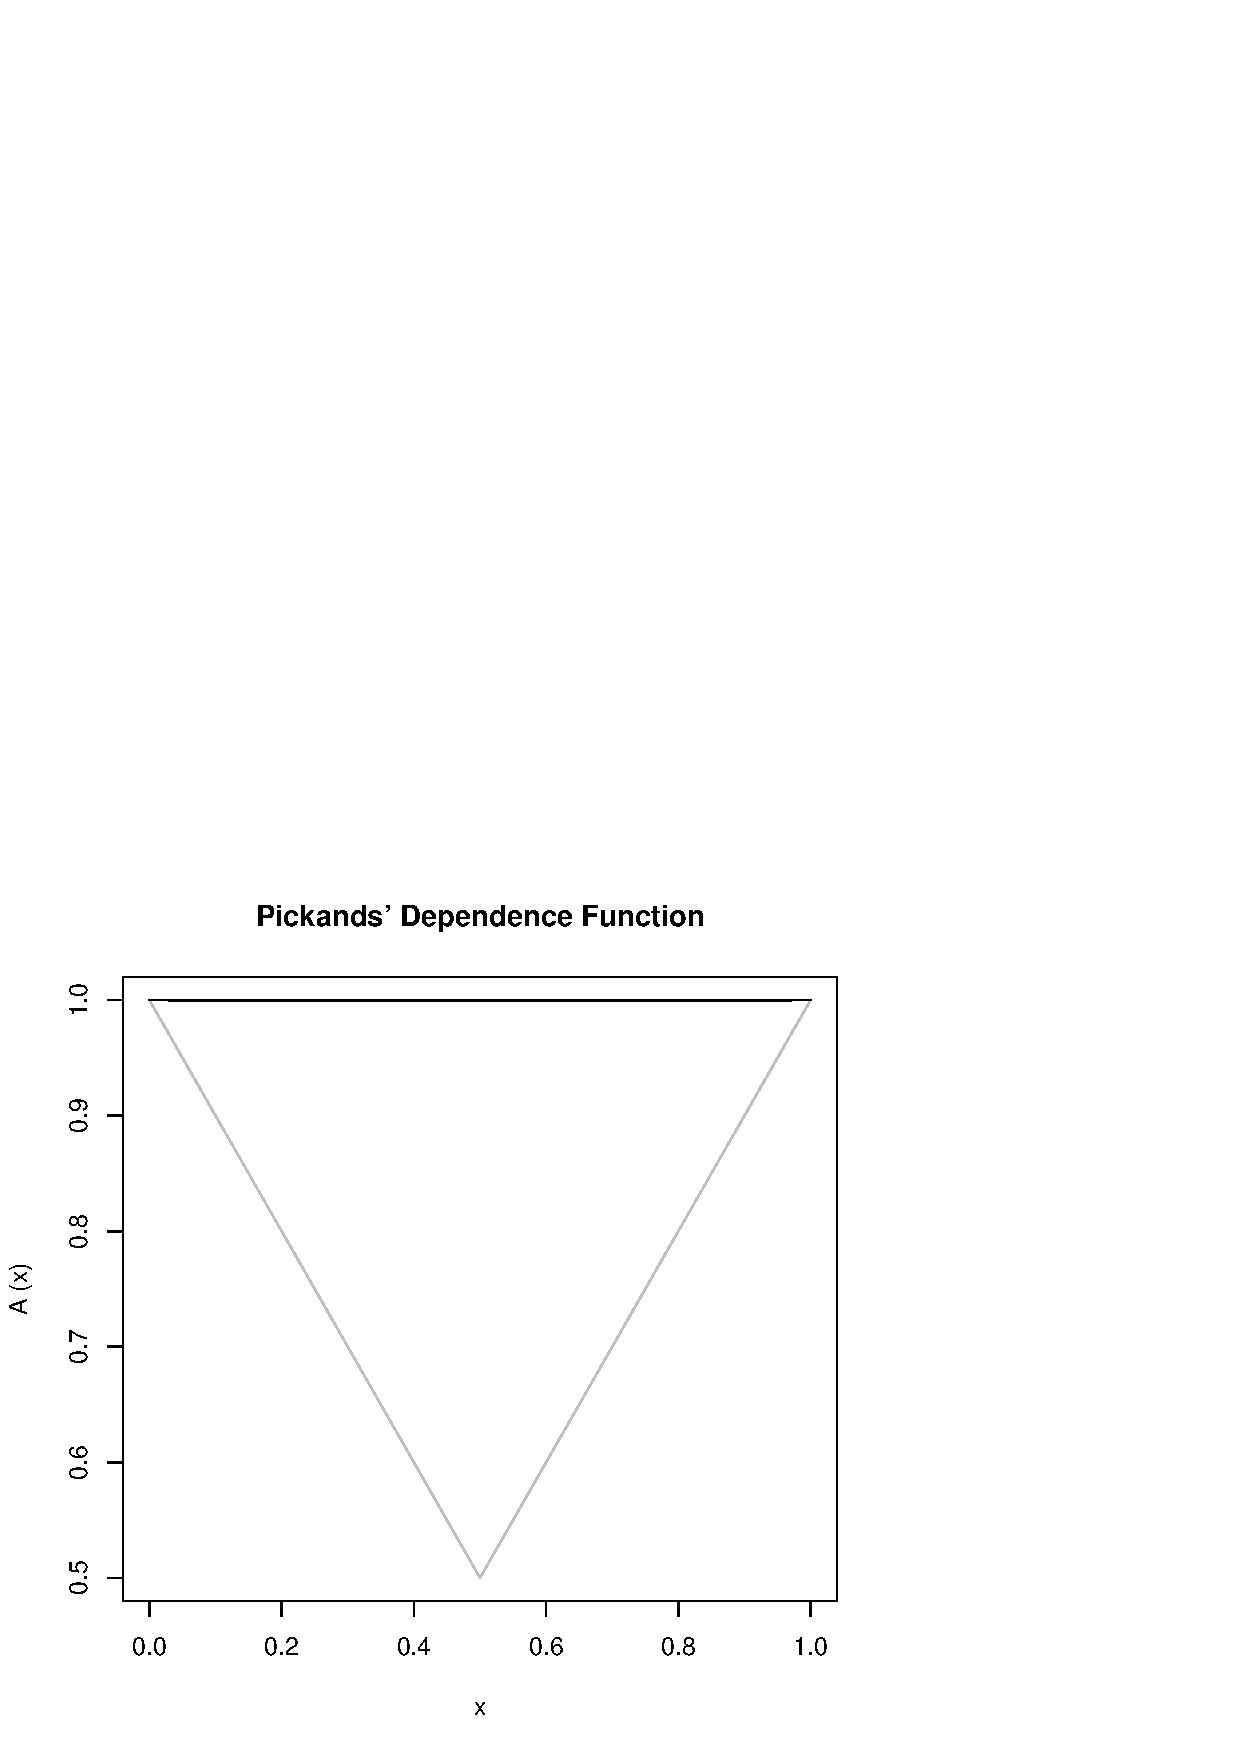
\includegraphics{guide-019}
\caption{The Pickands' dependence function}
\label{fig:pickdep}
\end{figure}

The horizontal line corresponds to independence while the
other ones corresponds to perfect dependence. Please note that by
construction, the \emph{mixed} and \emph{asymetric mixed} models can
not model perfect dependence variables.

\subsubsection{Markov Chains for Exceedances}

The classical way to perform an analysis of peaks over a threshold is
to fit the GPD to cluster maxima. However, there is a waste of data as
only the cluster maxima is considered. On the contrary, if we fit the
GPD to all exceedances, standard errors are underestimated as we
consider independence for dependent observations. Here is where Markov
Chains can help us. The main idea is to model the dependence structure
using a Markov Chains while the joint distribution is obviously a
multivariate extreme value distribution. This idea was first
introduces by~\citet{Smith1997}.

In the remainder of this section, we will only focus with first order
Markov Chains. Thus, the likelihood for all exceedances is:

\begin{equation}
  \label{eq:likMC}
  L(y_1, \ldots, y_n; \theta, \psi) = \frac{\prod_{i=2}^n
    f(y_{i-1},y_i;\theta, \psi)} {\prod_{i=2}^{n-1} f(y_i;\theta)}
\end{equation}
where $f(y_{i-1},y_i;\theta, \psi)$ is the joint density,
$f(y_i;\theta)$ is the marginal density, $\theta$ is the marginal GPD
parameters and $\psi$ is the dependence parameter. The marginals are
modelled using a GPD, while the joint distribution is a bivariate
extreme value distribution.

For our application, we use the \textbf{simmc} function which simulate
a first order Markov chain with extreme value dependence structure.
\begin{Schunk}
\begin{Sinput}
> mc <- simmc(1000, alpha = 0.5, model = "log")
> mc <- qgpd(mc, 2, 1, 0.15)
> fitmcgpd(mc, 2, "log")
\end{Sinput}
\begin{Soutput}
Call: fitmcgpd(data = mc, threshold = 2, model = "log") 
Estimator: MLE 
Dependence Model and Strenght:
	Model : Logistic 
	lim_u Pr[ X_1 > u | X_2 > u] = 0.607 
Deviance: 1501.887 
     AIC: 1507.887 

Threshold Call: 
Number Above: 998 
Proportion Above: 1 

Estimates
 scale   shape   alpha  
1.0459  0.1649  0.4784  

Standard Errors
  scale    shape    alpha  
0.11751  0.04247  0.02141  

Asymptotic Variance Covariance
       scale       shape       alpha     
scale   0.0138086  -0.0020998  -0.0015679
shape  -0.0020998   0.0018035  -0.0002175
alpha  -0.0015679  -0.0002175   0.0004585

Optimization Information
  Convergence: successful 
  Function Evaluations: 55 
  Gradient Evaluations: 12 
\end{Soutput}
\end{Schunk}


\subsection{Confidence Intervals}
\label{subsec:confInt}

Once a statistical model is fitted, it is usual to gives confidence
intervals. Currently, only \verb|mle|, \verb|pwmu|, \verb|pwmb|,
\verb|moments| estimators can computed confidence intervals. Moreover,
for method \verb|mle|, ``standard'' and ``profile'' confidence
intervals are available.

If we want confidence intervals for the scale parameters:
\begin{Schunk}
\begin{Sinput}
> x <- rgpd(200, 1, 2, 0.25)
> mle <- fitgpd(x, 1, method = "mle")
> mom <- fitgpd(x, 1, method = "moments")
> pwmb <- fitgpd(x, 1, method = "pwmb")
> pwmu <- fitgpd(x, 1, method = "pwmu")
> gpd.fiscale(mle, conf = 0.9)
\end{Sinput}
\begin{Soutput}
conf.inf.scale conf.sup.scale 
      1.762600       2.621287 
\end{Soutput}
\begin{Sinput}
> gpd.fiscale(mom, conf = 0.9)
\end{Sinput}
\begin{Soutput}
conf.inf.scale conf.sup.scale 
           NaN            NaN 
\end{Soutput}
\begin{Sinput}
> gpd.fiscale(pwmu, conf = 0.9)
\end{Sinput}
\begin{Soutput}
conf.inf.scale conf.sup.scale 
      1.751053       2.605097 
\end{Soutput}
\begin{Sinput}
> gpd.fiscale(pwmb, conf = 0.9)
\end{Sinput}
\begin{Soutput}
conf.inf.scale conf.sup.scale 
      1.763964       2.620164 
\end{Soutput}
\end{Schunk}

For shape parameter confidence intervals, simply use function
\verb|gpd.fishape| instead of \verb|gpd.fiscale|. Note that the
\emph{fi} stands for ``Fisher Information''.

Thus, if we want profile confidence intervals, we must use functions
\verb|gpd.pfscale| and \verb|gpd.pfshape|. The \emph{pf} stands for
``profile''. These functions are only available with a model fitted
with MLE.
\begin{Schunk}
\begin{Sinput}
> par(mfrow = c(1, 2))
> gpd.pfscale(mle, range = c(1, 2.9), conf = 0.9)
\end{Sinput}
\begin{Soutput}
If there is some troubles try to put vert.lines = FALSE or change
 the range...
conf.inf conf.sup 
1.796465 2.660101 
\end{Soutput}
\begin{Sinput}
> gpd.pfshape(mle, range = c(0, 0.6), conf = 0.85)
\end{Sinput}
\begin{Soutput}
If there is some troubles try to put vert.lines = FALSE or change
 the range...
 conf.inf  conf.sup 
0.2272727 0.5121212 
\end{Soutput}
\end{Schunk}

\begin{figure}
\centering
\begin{Schunk}
\begin{Soutput}
If there is some troubles try to put vert.lines = FALSE or change
 the range...
conf.inf conf.sup 
1.796465 2.660101 
\end{Soutput}
\begin{Soutput}
If there is some troubles try to put vert.lines = FALSE or change
 the range...
 conf.inf  conf.sup 
0.2272727 0.5121212 
\end{Soutput}
\end{Schunk}
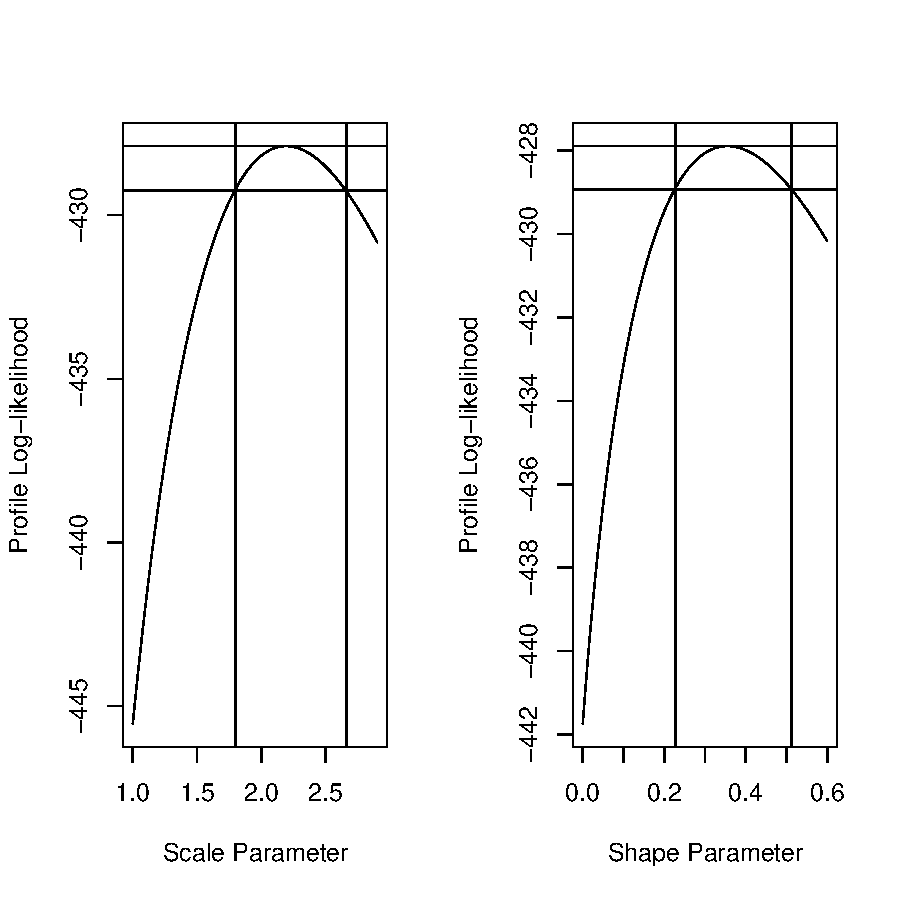
\includegraphics{guide-023}
\caption{The profile log-likelihood confidence intervals}
\label{fig:pfci}
\end{figure}

Confidence interval for quantiles - or return levels - are also
available. This is achieved using: (a) the Delta method or (b) profile
likelihood.
\begin{Schunk}
\begin{Sinput}
> gpd.firl(pwmu, prob = 0.95)
\end{Sinput}
\begin{Soutput}
conf.inf conf.sup 
12.07292 12.98166 
\end{Soutput}
\begin{Sinput}
> gpd.pfrl(mle, prob = 0.95, range = c(5, 16))
\end{Sinput}
\begin{Soutput}
If there is some troubles try to put vert.lines = FALSE or change
 the range...
conf.inf conf.sup 
10.27778 14.77778 
\end{Soutput}
\end{Schunk}

\begin{figure}
\centering
\begin{Schunk}
\begin{Soutput}
conf.inf conf.sup 
12.07292 12.98166 
\end{Soutput}
\begin{Soutput}
If there is some troubles try to put vert.lines = FALSE or change
 the range...
conf.inf conf.sup 
10.27778 14.77778 
\end{Soutput}
\end{Schunk}
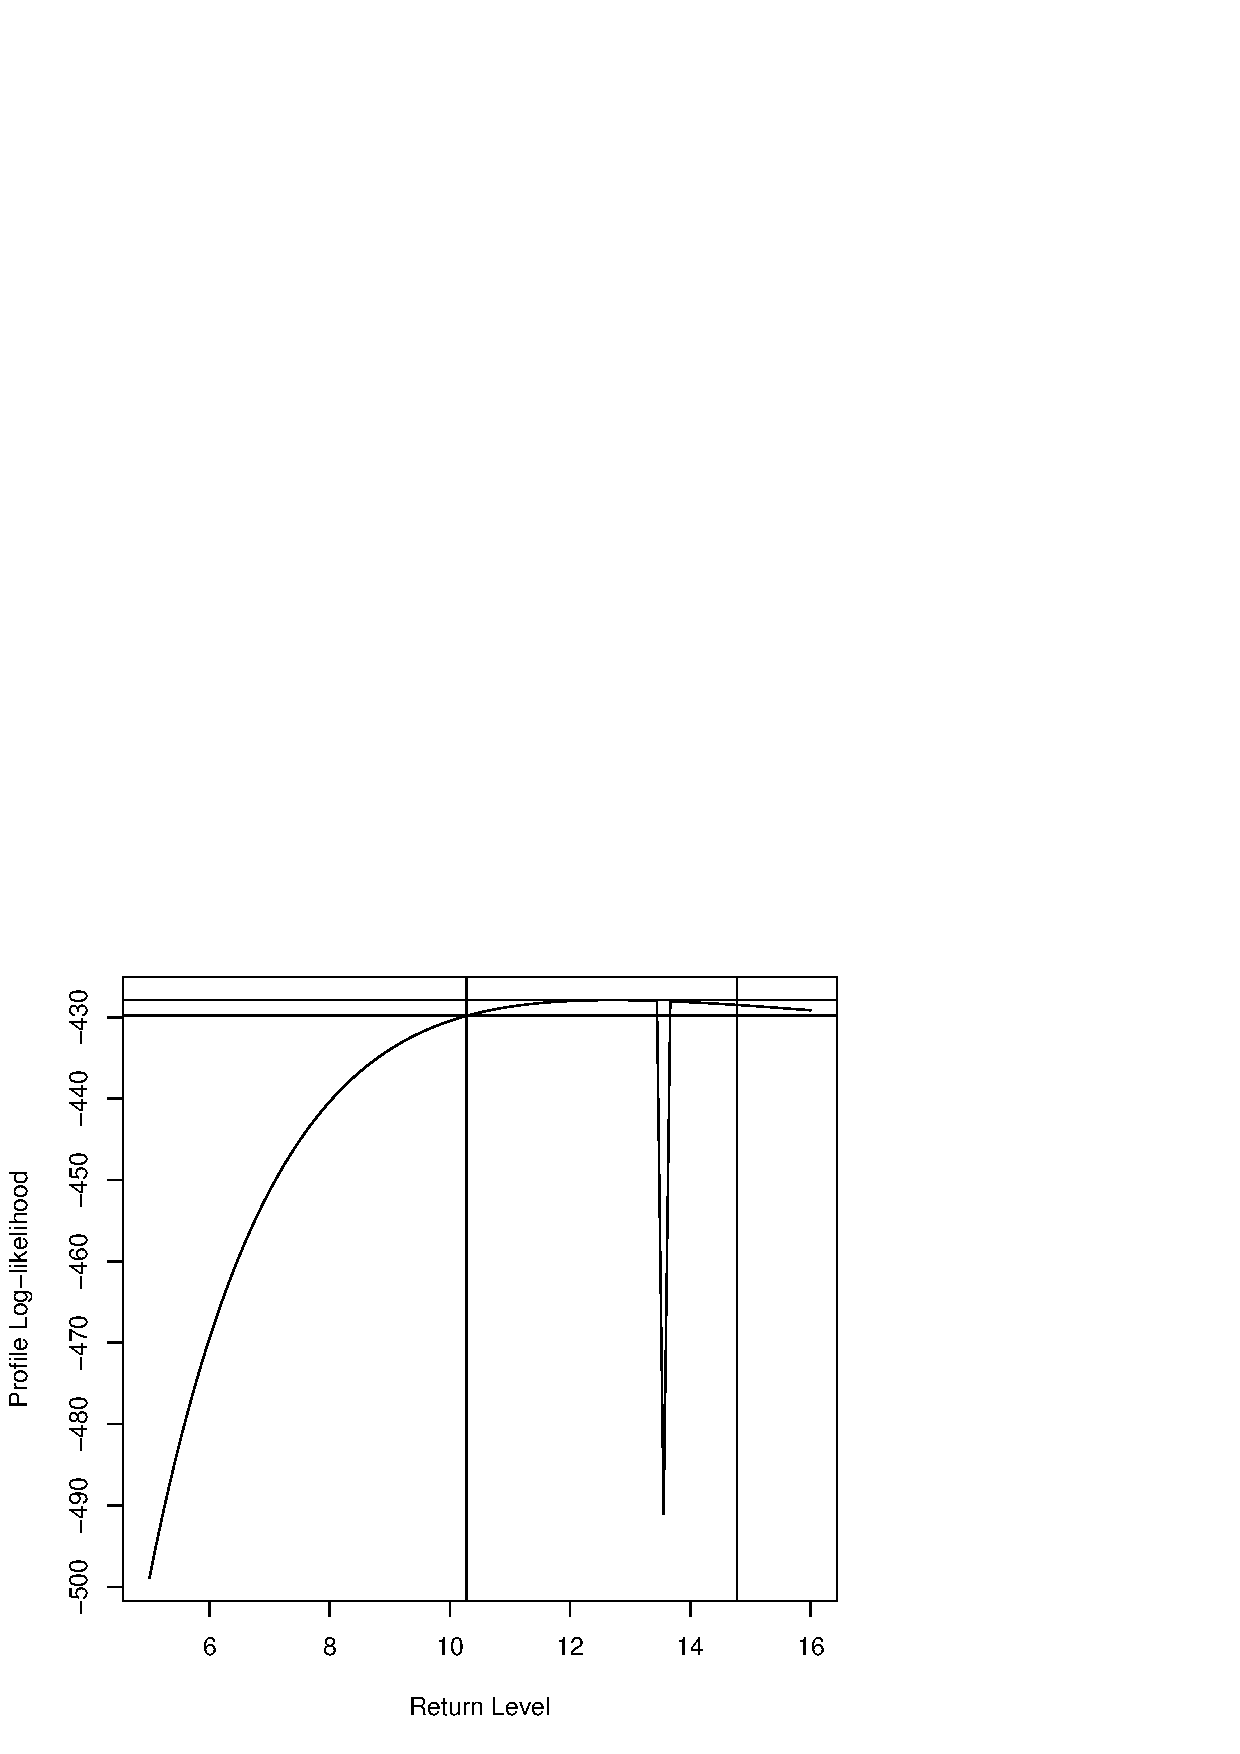
\includegraphics{guide-025}
\caption{The profile log-likelihood confidence interval for return
  levels} 
\label{fig:pfrl}
\end{figure}

The profile confidence interval functions both returns the confidence
interval and plot the profile log-likelihood
function. Figure~\ref{fig:pfrl} depicts the graphic window returned by
function \verb|gpd.pfrl| for the return level associated to non
exceedence probability 0.95.

\subsection{Model Checking}
\label{subsec:modCheck}


To check the fitted model, users must call function \textbf{plot}
which has a method for the \verb|uvpot|, \verb|bvpot| and \verb|mcpot|
classes. For example, this is a generic function which calls
functions: \verb|pp| (probability/probability plot), \verb|qq|
(quantile/quantile plot), \verb|dens| (density plot) and
\verb|retlev| (return level plot) for the uvpot class.

Here is a basic illustration of the function \verb|plot| for the class
\verb|uvpot|.
\begin{Schunk}
\begin{Sinput}
> x <- rgpd(200, 10, 0.5, -0.2)
\end{Sinput}
\end{Schunk}

\begin{Schunk}
\begin{Sinput}
> fitted <- fitgpd(x, 10, method = "mle")
> par(mfrow = c(2, 2))
> plot(fitted, npy = 1)
\end{Sinput}
\end{Schunk}

\begin{figure}
\centering
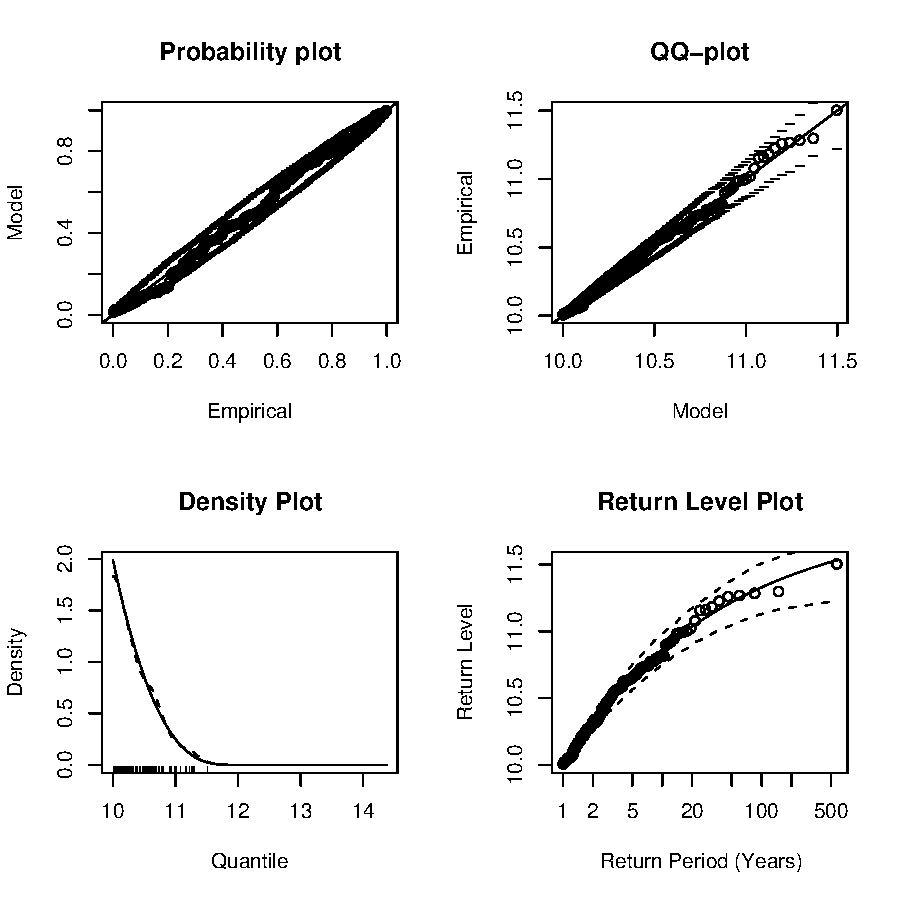
\includegraphics{guide-028}
\caption{Graphical diagnostic for a fitted POT model (univariate
  case)} 
\label{fig:plotgpd}
\end{figure}

Figure~\ref{fig:plotgpd} displays the graphic windows obtained with
the latter execution.

If one is interested in only a probability/probability plot, there is
two options. We can call function \verb|pp| or equivalently
\verb|plotgpd| with the \textbf{which} option. The ``which'' option
select which graph you want to plot. That is:
\begin{itemize}
\item{which = 1} for a probability/probability plot;
\item{which = 2} for a quantile/quantile plot;
\item{which = 3} for a density plot;
\item{which = 4} for a return level plot;
\end{itemize}
Note that ``which'' can be a vector like \verb|c(1,3)| or \verb|1:3|.

Thus, the following instruction gives the same graphic.

\begin{Schunk}
\begin{Sinput}
> plot(fitted, which = 1)
> pp(fitted)
\end{Sinput}
\end{Schunk}

If a return level plot is asked ($4 \in$ \verb|which|), a value for
\verb|npy| is needed. ``npy'' corresponds to the \emph{mean number of
  events per year}. This is required to define the ``return
period''. If missing, the default value (i.e. 1) will be chosen.

\subsection{Declustering Techniques}
\label{subsec:declust}

In opposition to block maxima, a peak over threshold can be
problematic when dealing with time series. Indeed, as often time
series are strongly auto-correlated, select naively events above a
threshold may lead to dependent events.

The function \textbf{clust} tries to identify peaks over a threshold
while meeting independence criteria. For this purpose, this function
needs at least two arguments: the threshold \verb|u| and a time
condition for independence \verb|tim.cond|. Clusters are identify as
follow:
\begin{enumerate}
\item The first exceedance initiates the first cluster;
\item The first observation under the threshold \verb|u| ``ends'' the
  cluster unless \verb|tim.cond| does not hold;
\item The next exceedance which hold \verb|tim.cond| initiates a new
  cluster;
\item The process is iterated as needed.
\end{enumerate}

Here is an application on flood discharges for river Ardi\`ere at
Beaujeu. A preliminary study shows that two flood events can be
considered independent if they do not lie within a 8 days window. Note
that unit to define \verb|tim.cond| must be the same than the data
analyzed. 
\begin{Schunk}
\begin{Sinput}
> data(ardieres)
> events <- clust(ardieres, u = 2, tim.cond = 8/365)
\end{Sinput}
\end{Schunk}

Several options can be passed to the ``clust'' function. By default,
it will return a list with the identified clusters. Usually, we want
only cluster maxima, this is achieved by passing option
\verb|clust.max = TRUE|. Users can also ask for a graphic
representation of clusters by passing option \verb|plot = TRUE| - see
Figure~\ref{fig:clust}.
\begin{Schunk}
\begin{Sinput}
> clustMax <- clust(ardieres, u = 2, tim.cond = 8/365, clust.max = TRUE, 
+     plot = TRUE, xlim = c(1971.1, 1972.9))
\end{Sinput}
\end{Schunk}
 

\begin{figure}
\centering
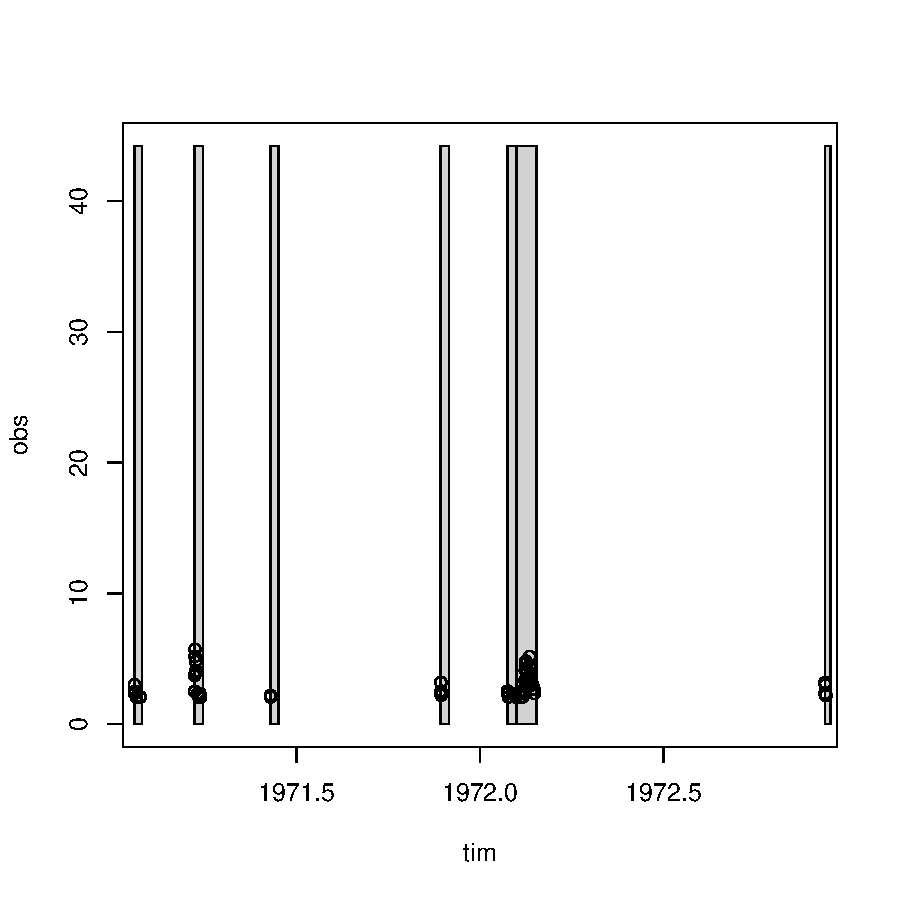
\includegraphics{guide-032}
\caption{The identified clusters. Data Ardi\`eres, u = 2, tim.cond = 8}
\label{fig:clust}
\end{figure}

\subsection{Miscellaneous functions}
\label{subsec:miscFunc}

\subsubsection{Return periods: \emph{rp2prob} and \emph{prob2rp}}

The functions \textbf{rp2prob} and \textbf{prob2rp} are useful to
convert return periods to non exceedence probabilities and vice
versa. It needs either a return period either a non exceedence
probability. Moreover, the mean number of events per year ``npy'' must
be specified.
\begin{Schunk}
\begin{Sinput}
> rp2prob(50, 1.8)
\end{Sinput}
\begin{Soutput}
  npy retper      prob
1 1.8     50 0.9888889
\end{Soutput}
\begin{Sinput}
> prob2rp(0.6, 2.2)
\end{Sinput}
\begin{Soutput}
  npy   retper prob
1 2.2 1.136364  0.6
\end{Soutput}
\end{Schunk}

\subsubsection{Unbiased Sample L-Moments: \emph{samlmu}}

The function \textbf{samlmu} computes the unbiased sample L-Moments.
\begin{Schunk}
\begin{Sinput}
> x <- runif(50)
> samlmu(x, nmom = 5)
\end{Sinput}
\begin{Soutput}
         l_1          l_2          t_3          t_4          t_5 
 0.446092724  0.172668876  0.148438038 -0.008121012 -0.074447794 
\end{Soutput}
\end{Schunk}

\subsubsection{Mobile average window on time series: \emph{ts2tsd}}

The function \textbf{ts2tsd} computes an ``average'' time series
\verb|tsd| from the initial time series \verb|ts|. This is achieved by
using a mobile average window of length \verb|d| on the initial time
series.
\begin{Schunk}
\begin{Sinput}
> data(ardieres)
> tsd <- ts2tsd(ardieres, 3/365)
> plot(ardieres, type = "l", col = "blue")
> lines(tsd, col = "green")
\end{Sinput}
\end{Schunk}

The latter execution is depicted in Figure~\ref{fig:ts2tsd}.
\begin{figure}
\centering
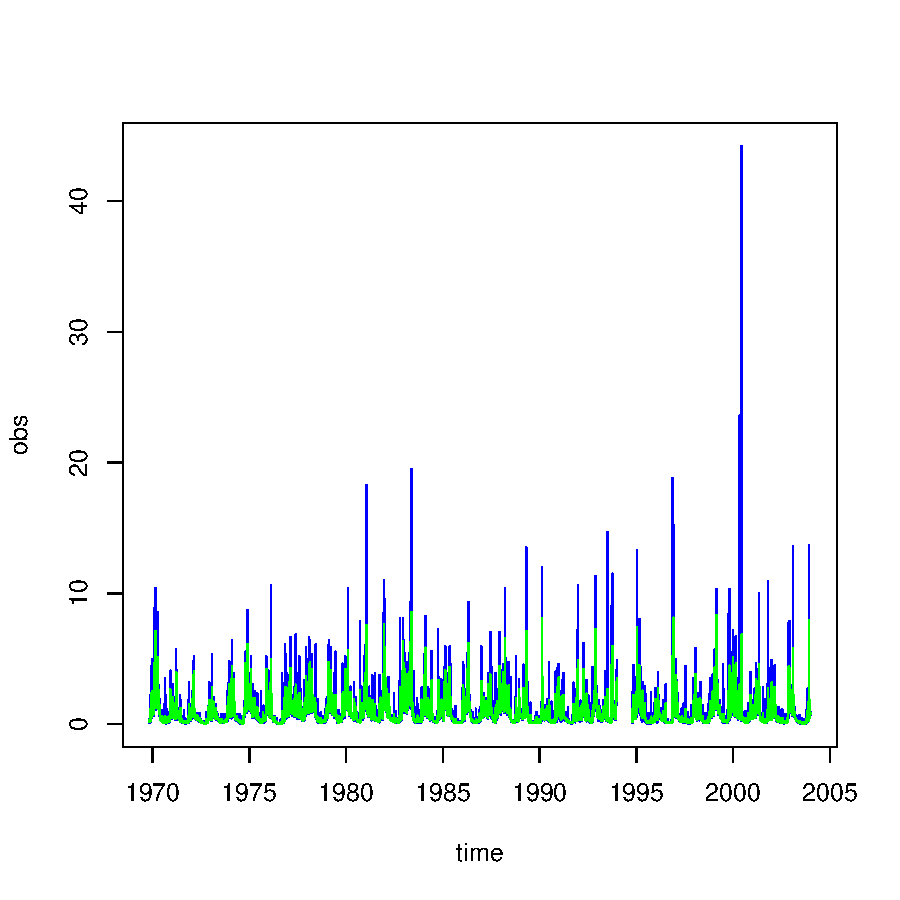
\includegraphics{guide-036}
\caption{Instantaneous flood discharges and averaged dischaged over
  duration 3 days. Data ardieres}
\label{fig:ts2tsd}
\end{figure}

\section{A Concrete Statistical Analysis of Peaks Over a Threshold}
\label{sec:concAn}

In this section, we provide a full and detailed analysis of peaks over
a threshold for the river Ardi\`eres at
Beaujeu. Figure~\ref{fig:ts2tsd} depicts instantaneous flood
discharges - blue line.

As this is a time series, we must selects independent events above a
threshold. First, we fix a relatively low threshold to ``extract''
more events. Thus, some of them are not extreme but regular
events. This is necessary to select a reasonable threshold for the
asymptotic approximation by a GPD - see section~\ref{sec:introEVT}.
\begin{Schunk}
\begin{Sinput}
> summary(ardieres)
\end{Sinput}
\begin{Soutput}
      time           obs        
 Min.   :1970   Min.   : 0.022  
 1st Qu.:1981   1st Qu.: 0.236  
 Median :1991   Median : 0.542  
 Mean   :1989   Mean   : 1.024  
 3rd Qu.:1997   3rd Qu.: 1.230  
 Max.   :2004   Max.   :44.200  
                NA's   : 1.000  
\end{Soutput}
\begin{Sinput}
> events0 <- clust(ardieres, u = 1.5, tim.cond = 8/365, clust.max = TRUE)
> par(mfrow = c(2, 2))
> mrlplot(events0[, "obs"])
> abline(v = 6, col = "green")
> diplot(events0)
> abline(v = 6, col = "green")
> tcplot(events0[, "obs"], which = 1)
> abline(v = 6, col = "green")
> tcplot(events0[, "obs"], which = 2)
> abline(v = 6, col = "green")
\end{Sinput}
\end{Schunk}

From Figure~\ref{fig:threshSelect}, a threshold value of $6 m^3/s$
should be reasonable. The Mean residual life plot - top left panel-
indicates that a threshold around $10 m^3/s$ should be
adequate. However, the selected threshold must be low enough to have
enough events above it to reduce variance while not too low as it
increase the bias\footnote{As the asymptotic approximation by a GPD is
  not accurate anymore.}.

\begin{figure}
\centering
\begin{Schunk}
\begin{Soutput}
      time           obs        
 Min.   :1970   Min.   : 0.022  
 1st Qu.:1981   1st Qu.: 0.236  
 Median :1991   Median : 0.542  
 Mean   :1989   Mean   : 1.024  
 3rd Qu.:1997   3rd Qu.: 1.230  
 Max.   :2004   Max.   :44.200  
                NA's   : 1.000  
\end{Soutput}
\end{Schunk}
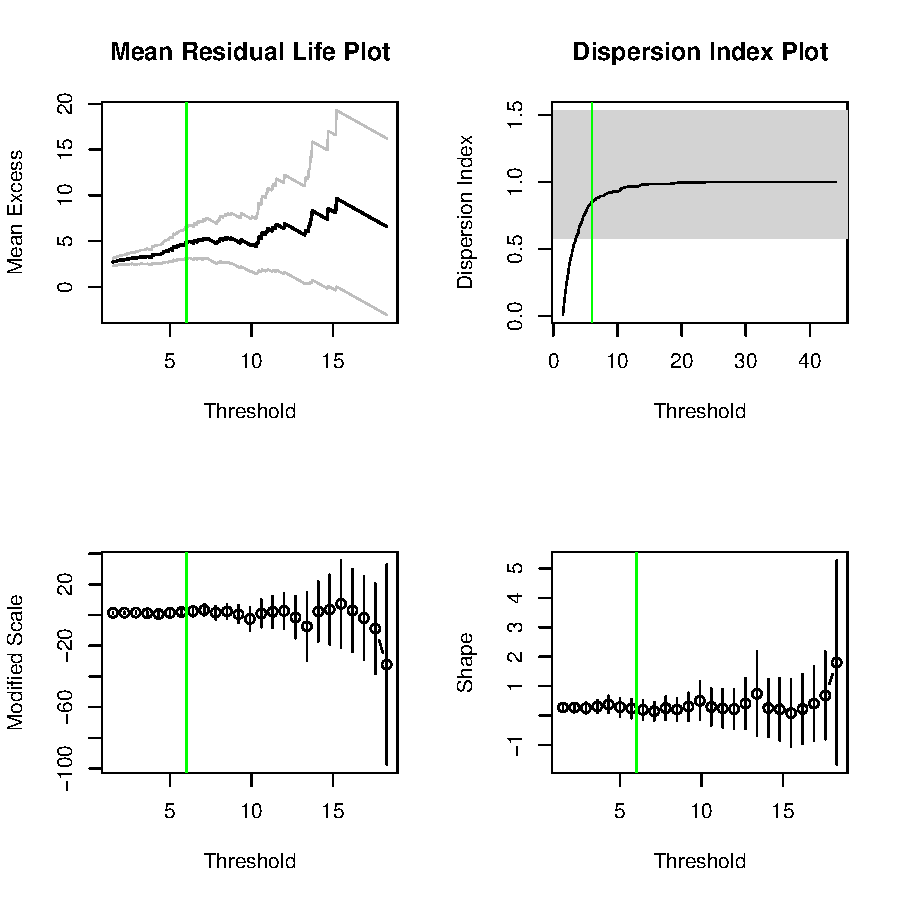
\includegraphics{guide-038}
\caption{Threshold selection for river Ardi\`eres at Beaujeu.}
\label{fig:threshSelect}
\end{figure}

Thus, we can now ``re-extract'' events above the threshold $6 m^3/s$,
obtaining object \verb|events1|. This is necessary as sometimes
\verb|events1| is not equal to observations of \verb|events0| greater
than $6 m^3/s$. We can now define the mean number of events per year
``npy''. Note that an estimation of the extremal index is available.
\begin{Schunk}
\begin{Sinput}
> events1 <- clust(ardieres, u = 6, tim.cond = 8/365, clust.max = TRUE)
> npy <- length(events1[, "obs"])/(diff(range(ardieres[, "time"], 
+     na.rm = TRUE)) - diff(ardieres[c(20945, 20947), "time"]))
> print(npy)
\end{Sinput}
\begin{Soutput}
[1] 1.707897
\end{Soutput}
\begin{Sinput}
> attributes(events1)$exi
\end{Sinput}
\begin{Soutput}
[1] 0.1247265
\end{Soutput}
\end{Schunk}

Let's fit the GPD.
\begin{Schunk}
\begin{Sinput}
> mle <- fitgpd(events1[, "obs"], thresh = 6, method = "mle")
> par(mfrow = c(2, 2))
> plot(mle, npy = npy)
\end{Sinput}
\end{Schunk}

The result of function \textbf{fitgpd} gives the name of the
estimator, if a varying threshold was used, the threshold value, the
number and the proportion of observations above the threshold,
parameter estimates, standard error estimates and type, the asymptotic
variance-covariance matrix and convergence diagnostic.

\begin{figure}
\centering
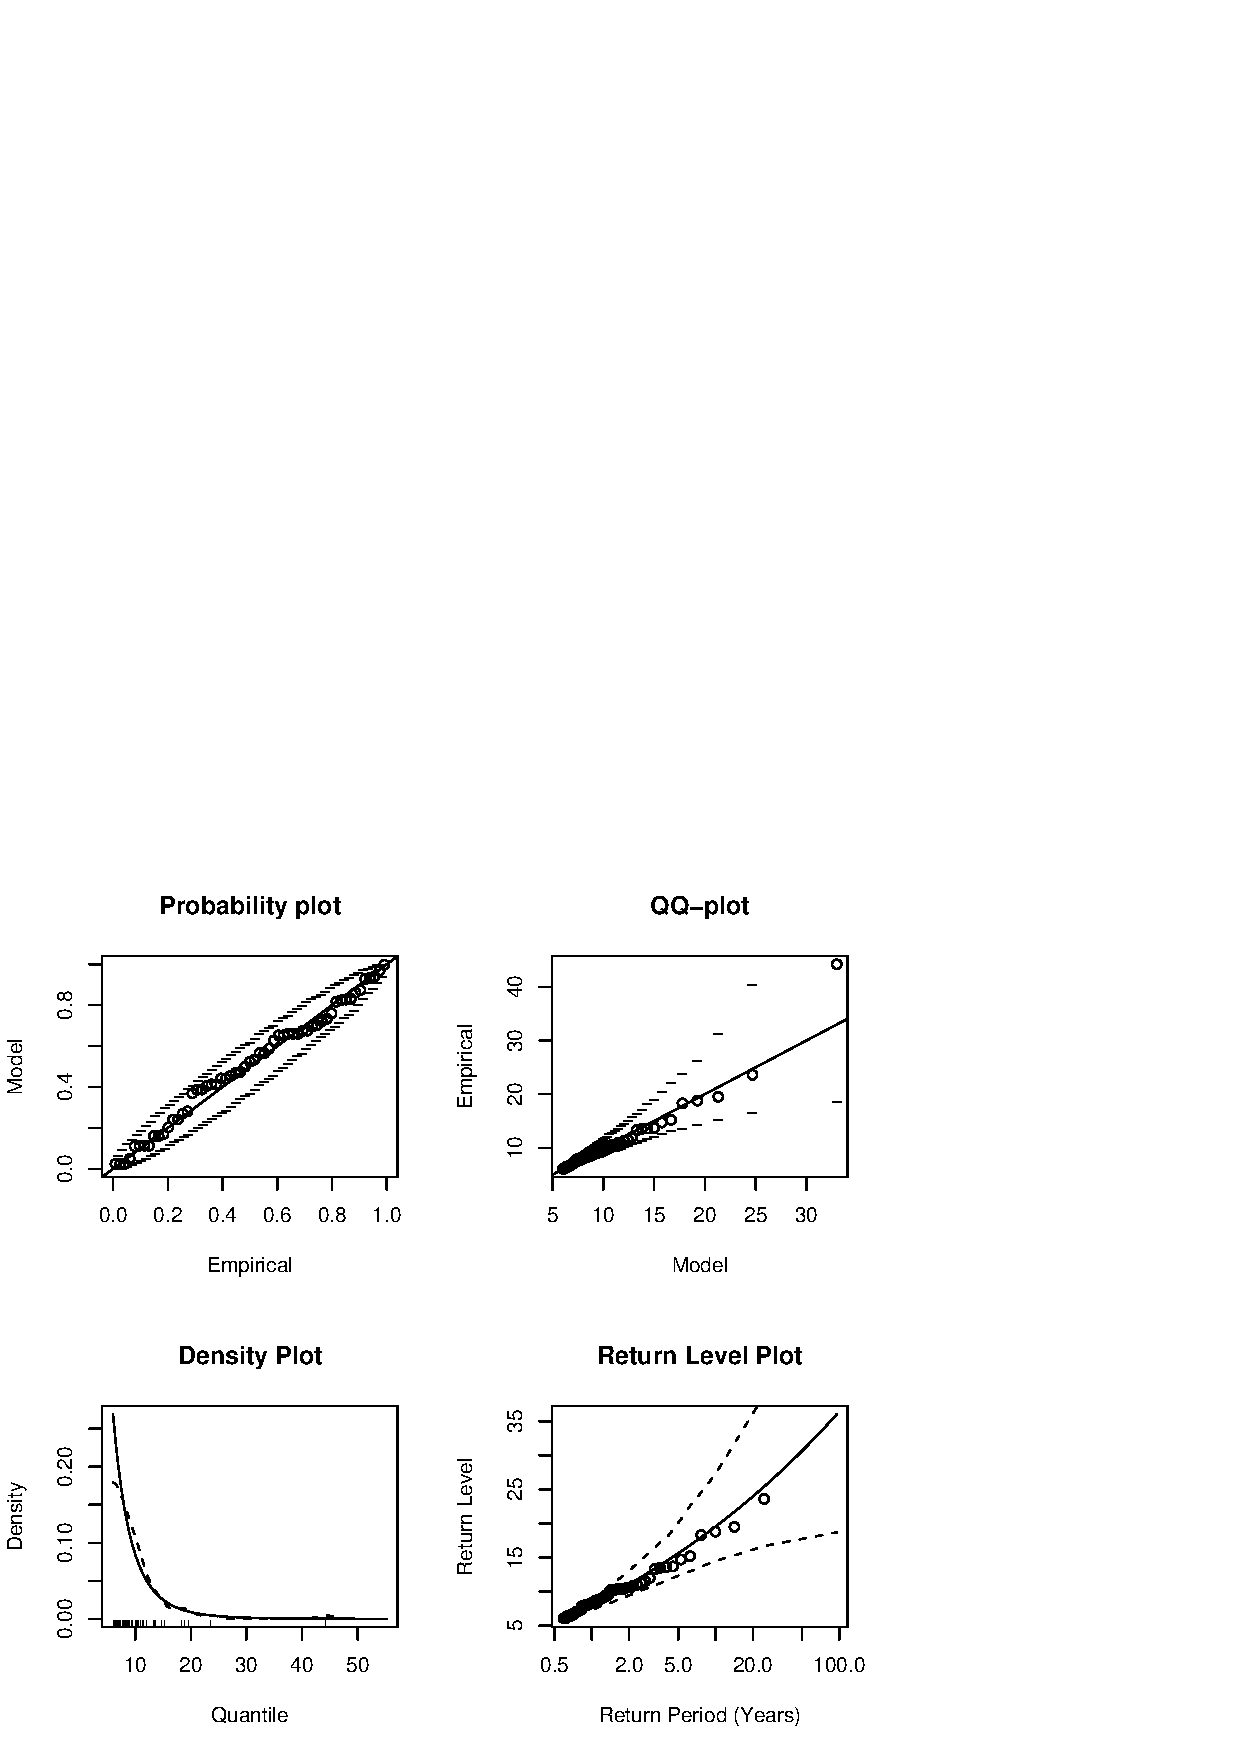
\includegraphics{guide-041}
\caption{Graphic diagnostics for river Ardi\`eres at Beaujeu}
\label{fig:checkArdieres}
\end{figure}

Figure~\ref{fig:checkArdieres} shows graphic diagnostics for the
fitted model. It can be seen that the fitted model ``mle'' seems to be
appropriate. Suppose we want to know the return level associated to
the 100-year return period.
\begin{Schunk}
\begin{Sinput}
> rp2prob(retper = 100, npy = npy)
\end{Sinput}
\begin{Soutput}
       npy retper      prob
1 1.707897    100 0.9941448
\end{Soutput}
\begin{Sinput}
> prob <- rp2prob(retper = 100, npy = npy)[, "prob"]
> qgpd(prob, loc = 6, scale = mle$param["scale"], shape = mle$param["shape"])
\end{Sinput}
\begin{Soutput}
   scale 
36.44331 
\end{Soutput}
\end{Schunk}

To take into account uncertainties, Figure~\ref{fig:pfrlArdieres}
depicts the profile confidence interval for the quantile associated to
the 100-year return period.
\begin{Schunk}
\begin{Sinput}
> gpd.pfrl(mle, prob, range = c(25, 100), nrang = 200)
\end{Sinput}
\begin{Soutput}
If there is some troubles try to put vert.lines = FALSE or change
 the range...
conf.inf conf.sup 
25.56533 90.76633 
\end{Soutput}
\end{Schunk}

\begin{figure}
\centering
\begin{Schunk}
\begin{Soutput}
If there is some troubles try to put vert.lines = FALSE or change
 the range...
conf.inf conf.sup 
25.56533 90.76633 
\end{Soutput}
\end{Schunk}
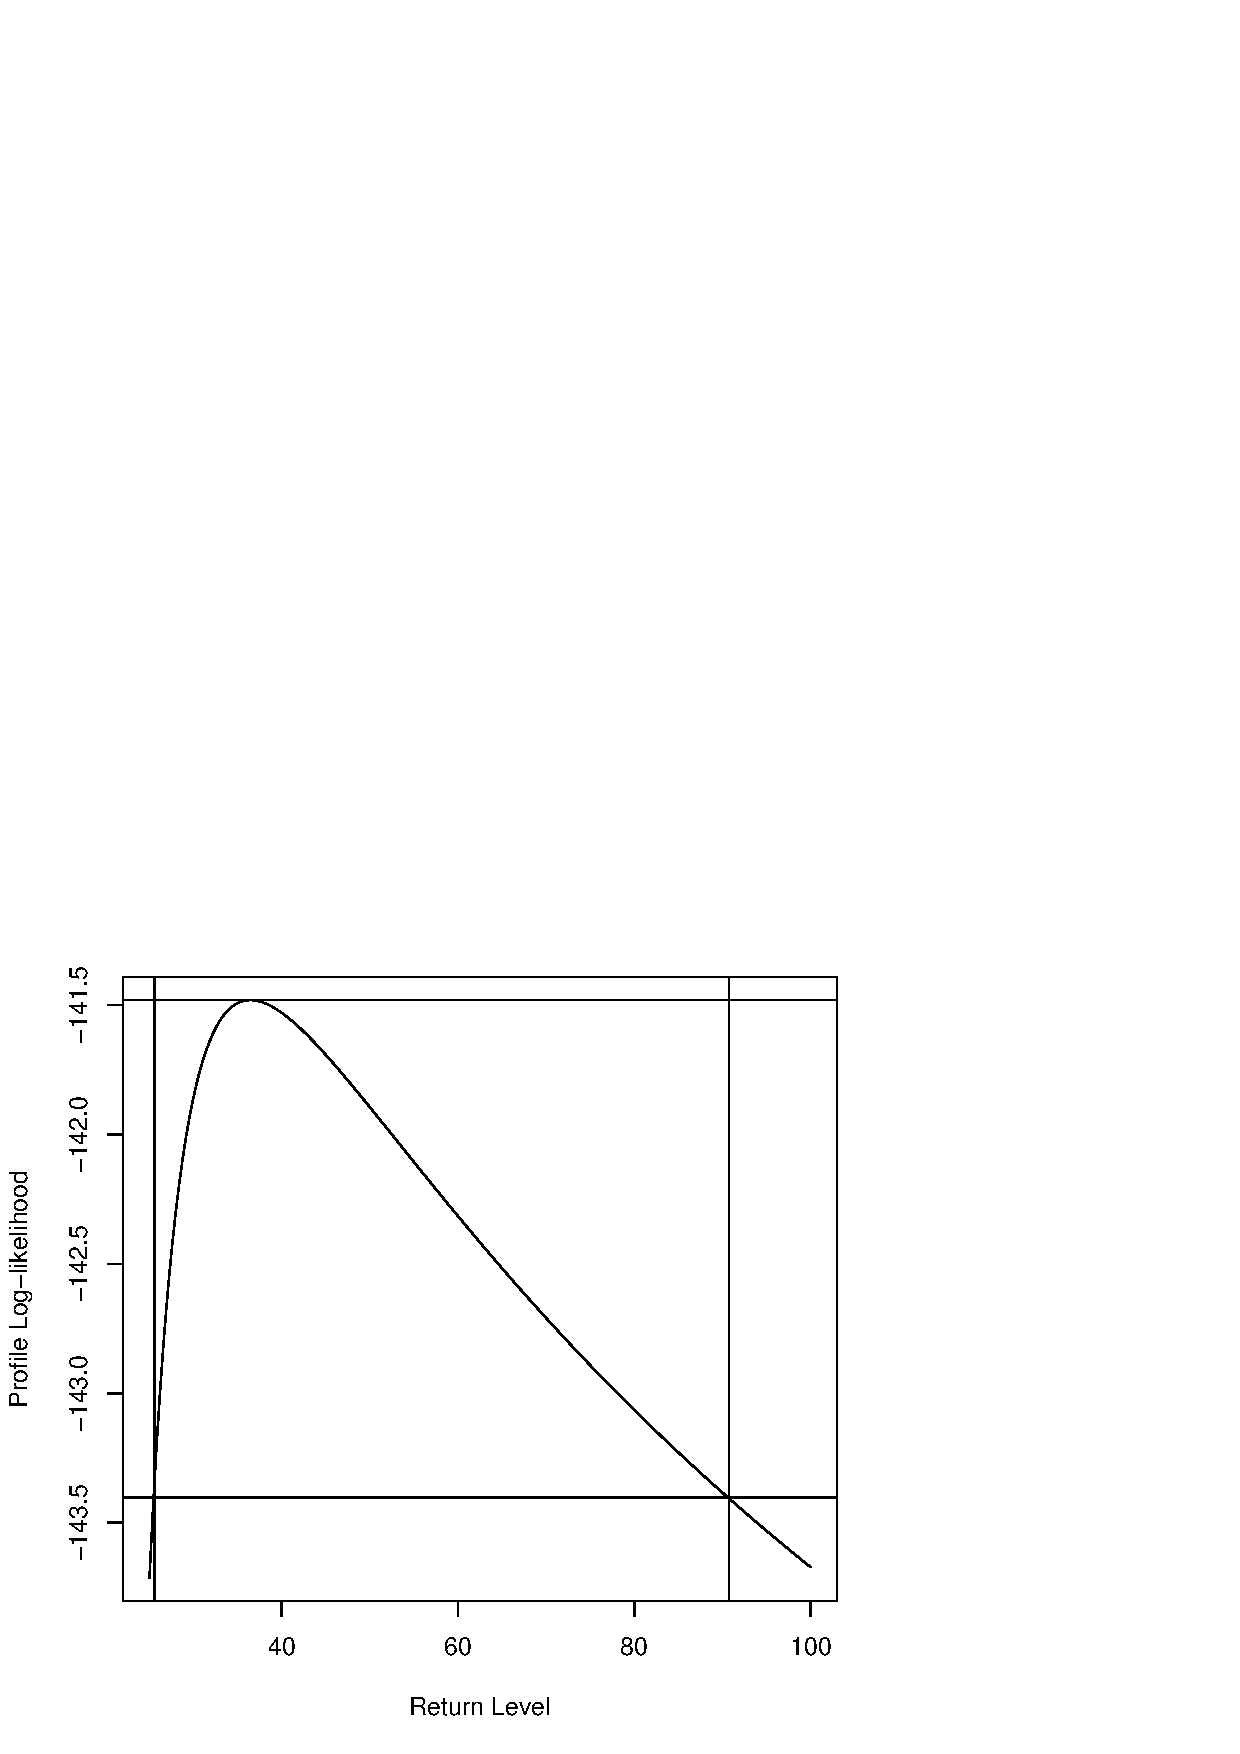
\includegraphics{guide-044}
\caption{Profile-likelihood function for the 100-year return period
  quantile} 
\label{fig:pfrlArdieres}
\end{figure}

Sometimes it is necessary to know the estimated return period of a
specified events. Lets do it with the larger events in ``events1''.
\begin{Schunk}
\begin{Sinput}
> maxEvent <- max(events1[, "obs"])
> maxEvent
\end{Sinput}
\begin{Soutput}
[1] 44.2
\end{Soutput}
\begin{Sinput}
> prob <- pgpd(maxEvent, loc = 6, scale = mle$param["scale"], shape = mle$param["shape"])
> prob
\end{Sinput}
\begin{Soutput}
    shape 
0.9974115 
\end{Soutput}
\begin{Sinput}
> prob2rp(prob, npy = npy)
\end{Sinput}
\begin{Soutput}
       npy   retper      prob
1 1.707897 226.1982 0.9974115
\end{Soutput}
\end{Schunk}

Thus, the largest events that occurs in June 2000 has approximately a
return period of 240 years.

Maybe it is a good idea to fit the GPD with the other estimators
available in the \textbf{POT} package.

\clearpage
\appendix

\section{Dependence Models for Bivariate Extreme Value
  Distributions}
\label{sec:copula}

\subsection{The Logisitic model}

The logisitic model is defined by:
\begin{equation}
  \label{eq:logistic}
  V(x,y) = \left( x^{-1/\alpha} + y^{-1/\alpha} \right)^\alpha, \qquad
  0 < \alpha \leq 1 
\end{equation}

Independence is obtained when $\alpha = 1$ while total dependence for
$\alpha \rightarrow 0$.

The Pickands' dependence function for the logistic model is:
\begin{eqnarray*}
  A: \left[0,1\right] &\longrightarrow& \left[0,1\right]\\
  w &\longmapsto& \left[\left(1-w\right)^\frac{1}{\alpha} +
    w^\frac{1}{\alpha} \right]^\alpha
\end{eqnarray*}

\subsection{The Asymetric Logistic model}

The asymetric logistic model is defined by:
\begin{displaymath}
  V(x,y) = \frac{1 - \theta_1}{x} + \frac{1 - \theta_2}{y} + \left[
    \left(\frac{x}{\theta_1} \right)^{-\frac{1}{\alpha}} +
      \left(\frac{y}{\theta_2} \right)^{-\frac{1}{\alpha}}
    \right]^\alpha,
\end{displaymath}
with $0 < \alpha \leq 1$, $0 \leq \theta_1, \theta_2 \leq 1$.

Independence is obtained when either $\alpha=1$, $\theta_1=0$ or
$\theta_2=0$. Differents limits occur when $\theta_1$ and $\theta_2$
are fixed and $\alpha=1 \rightarrow 0$.

The Pickands' dependence function for the asymetric logistic model is:
\begin{displaymath}
  A(w) = \left(1 - \theta_1 \right) \left(1 - w\right) +  \left(1 -
    \theta_2 \right) w + \left[ (1 - w)^{\frac{1}{\alpha}}
    \theta_1^{\frac{1}{\alpha}} + w^{\frac{1}{\alpha}}
    \theta_2^{\frac{1}{\alpha}} \right]^{\alpha}
\end{displaymath}

\subsection{The Negative Logistic model}

The negative logistic model is defined by:
\begin{equation}
  \label{eq:negLog}
  V(x,y) = \frac{1}{x} + \frac{1}{y} - \left(x^{\alpha} + y^{\alpha}
  \right)^{-\frac{1}{\alpha}}, \qquad \alpha > 0
\end{equation}

Independence is obtained when $\alpha \rightarrow 0$ while total
dependence when $\alpha \rightarrow +\infty$. 

The Pickands' dependence function for the negative logistic model is:
\begin{displaymath}
  A(w) = 1 - \left[ (1 - w)^{-\alpha} + w^{-\alpha}
  \right]^{-\frac{1}{\alpha}}
\end{displaymath} 

\subsection{The Asymetric Negative Logistic model}

The asymetric negative logistic model is defined by:
\begin{displaymath}
  V(x,y) = \frac{1}{x} + \frac{1}{y} - \left[ \left(\frac{x}{\theta_1}
    \right)^\alpha  + \left(\frac{y}{\theta_2} \right)^\alpha
  \right]^{-\frac{1}{\alpha}}, \qquad \alpha > 0, \quad 0 <
  \theta_1, \theta_2 \leq 1
\end{displaymath}

Independence is obtained when either $\alpha \rightarrow 0$, $\theta_1
\rightarrow 0$ or $\theta_2 \rightarrow 0$. Different limits occur
when $\theta_1$ and $\theta_2$ are fixed and $\alpha \rightarrow
+\infty$.

The Pickands' dependence function for the asymetric negative logistic
model is:
\begin{displaymath}
  A(w) = 1 - \left[ \left(\frac{1 - w}{\theta_1} \right)^{-\alpha} + 
    \left(\frac{w}{\theta_2} \right)^{-\alpha}
  \right]^{-\frac{1}{\alpha}}
\end{displaymath}

\subsection{The Mixed model}

The mixed model is defined by:
\begin{displaymath}
  V(x,y) = \frac{1}{x} + \frac{1}{y} - \frac{\alpha}{x+y}, \qquad 0
  \leq \alpha \leq 1
\end{displaymath}

Independence is obtained when $\alpha = 0$ while total dependence
could never be reached.

The Pickands' dependence function for the mixed model is:
\begin{displaymath}
  A(w) = 1 - w  \left(1 -w\right) \alpha
\end{displaymath}

\subsection{The Asymetric Mixed model}

The asymetric mixed model is defined by:
\begin{displaymath}
  V(x,y) = \frac{1}{x} + \frac{1}{y} - \frac{\left( \alpha + \theta
    \right) x + \left(\alpha + 2\theta \right) y}{\left( x+ y
    \right)^2}, \qquad \alpha \geq 0,\quad \alpha + 2 \theta \leq 1,
  \quad  \alpha + 3\theta \geq 0
\end{displaymath}

Independence is obtained when $\alpha = \theta = 0$ while total
dependence could never be reached.

The Pickands' dependence function for the asymetric mixed model is:
\begin{displaymath}
  A(w) = \theta w^3 + \alpha w^2 - \left(\alpha + \theta \right) w +
  1
\end{displaymath}


\bibliography{e:/Docs/LateX/biblio_ribatet}
\end{document}
%%% Local Variables: 
%%% mode: latex
%%% TeX-master: t
%%% End: 
